% !TEX root = ../thesis-example.tex
%
\chapter{Instances éphémères d'agencements modulaires}
\label{ch:ephemeral}

% \cleanchapterquote{Paradoxalement, la musique du futur est écrite sur du sable!}{Michel Chion}{La musique du futur a-t-elle un avenir?, 1977}

%\cleanchapterquote{Le vieux Paris n'est plus (la forme d'une ville\\
%Change plus vite, hélas ! que le coeur d'un mortel)}{Charles Baudelaire}{Le Cygne, 1861}

\cleanchapterquote{La musique (...) est trop en deçà du monde\\
et du désignable pour figurer autre chose\\
que des épures de l'Être, son flux et son reflux,\\
sa croissance, ses éclatements, ses tourbillons.}
{Maurice Merleau-Pontry}{L'Œil et l'Esprit, 1964} %\cite{merleau-ponty_loeil_1964}

%\cleanchapterquote{Dufourt suggests that contemporary music\\
%highlights what was rejected in the Greek world:\\
%it rather captures the evanescent, the ephemeral,\\
%the ambivalent, the Erebus, it favors the endless\\
%metamorphosis of qualities and forms;\\
%as Nietzsche proclaimed, western music tends\\
%toward the liberation of the dyonisiac dimension\\
%and the acceptance of the inacceptable part of myths.}
%{Jean-Claude Risset}{Discours invité à la conférence ICMC, 2014}%\cite{risset_sound_2014} % Remettre cette citation dans le corps du texte.

\vspace*{\fill}

\noindent Nous avons exposé dans le préambule le fait que l'instrument de musique ne se laisse pas facilement définir, tant la notion de musique est sujette à des interprétations diverses, et que l'apport du numérique sembler venir brouiller davantage encore les définitions et contours de l'objet. L'expression \textit{digital musical instrument}, dont l'usage croissant depuis le tournant du millénaire a fini par la condenser en l'acronyme \gls{DMI}, pourrait nous laisser croire, a contrario, qu'une forme certes mal-définie se cristallise. Pourtant, il semble que ce soit l'\textit{éphémérité}, ou l'\textit{obsolescence} des \glspl{DMI} (selon la perspective optimiste ou pessimiste que l'on adopte) qui les caractérisent, davantage qu'une stabilité effective, et qui se traduit par un souci croissant de la question de leur pérennité.
\indent Après un rapide historique de l'émergence des \gls{DMI}, j'analyserai dans ce chapitre les termes de leur instabilité, dans la perspective de ce qu'ils impliquent comme choix et méthodes adaptés pour la conception et la pratique.

\clearpage

%\test{blabla}
\section{Paysage des DMIs}
\label{sec:ephemerality:landscape}

%--------------------------------------------------------------
\subsection{Les origines}
\label{sec:ephemeral:origins}

\subsubsection{Pré-histoire}
\label{sec:ephemeral:origins:prehistory}

\noindent Les instruments acoustiques héritent d'une histoire vieille de plus de 40~000ans \cite{conard_new_2009} et la finesse de leur fabrication a atteint une excellence qui fait de certains instruments de véritables pièces d'orfèvres. Les instruments numériques, beaucoup plus récents en comparaison, ne peuvent rivaliser avec ce degré de raffinement. Pour autant, il ne sont pas totalement déshérités de la tradition et du savoir-faire des instruments acoustiques et, par ailleurs, le développement hautement collaboratif à l'œuvre dans le domaine de la programmation informatique leur confère, malgré leur jeunesse, une grande complexité — les compétences requises pour la fabrication d'un \gls{DMI} de A à Z dépassant souvent largement ce qu'il serait possible pour un individu seul de concevoir. C'est en effet un trait caractéristique des objets techniques de l'ère post-industrielle que d'être le produit du travail d'un très grand nombre d'individus\footnote{Un exemple notoire en fut donné par l'économiste Leonard Read (et repris par Milton Friedman) dans l'essai ``I, pencil''\cite{read_i_1958}, prenant l'exemple d'un simple crayon à papier pour démontrer que des millions de gens avait collaboré à sa fabrication.} et d'être assemblés à partir d'éléments de base déjà manufacturés et complexes.\\
\indent Parmi les diverses caractéristiques des \glspl{DMI}, la plus notable est probablement le découplage total entre le geste du musicien et le son. Ce découplage énergétique et plus généralement, l'extériorisation du travail dans les outils, est un processus ancien qui a été en particulier analysé par le paléo-anthropologue André Leroi-Gourhan \cite{leroi-gourhan_geste_1964}. En ce qui concerne les instruments, on observe des ruptures dans l'histoire de la lutherie au moment de grandes avancées scientifiques et technologique. Jean-Claude Risset note en particulier dans \cite{genevois_les_1999} la naissance de l'orgue comme un moment charnière, au regard des questions qui m'intéressent ici: \iquote{L'orgue marque le rôle croissant de la technologie dans l'instrument de musique: il introduit le premier interrupteur, le premier clavier, et dès le \siecle{15}~siècle la première synthèse additive (qui ne sera justifiée mathématiquement par Fourier qu'au \siecle{19}~siècle). L'orgue est aussi la première machine informationnelle: l'information donnée par le geste du musicien y est décuplée de l'énergie sonore.}\footnote{On notera au passage que le terme ``décuplé'', qui semble être une coquille (intentionnelle ?) du terme ``découplé'', reste tout à fait pertinent!}\\
\indent La révolution industrielle est un autre moment charnière, une période de nombreux développements qui anticipent les révolutions technologiques du \siecle{20}~siècle. On notera notamment les progrès mécaniques: les machines-outils permettent la réalisation de pièces mécaniques de plus en plus précises et fabriquées en grande série. Cela donnera lieu notamment à des systèmes tels que le clétage de Boehm, qui permet le déport des doigts et révolutionne la famille des instruments à vent. Enfin (et surtout), l'arrivée concomittente de la téléphonie et de l'enregistrement dans la seconde moitié du \siecle{19}~siècle, qui déportent la production sonore dans l'espace et dans le temps et seront les vecteurs d'une transformation profonde de la société, et en particulier pour ce qui nous intéresse ici, des modes de production et de réception de la musique\footnote{Sur ce vaste sujet, voir en particulier~\cite{theberge_any_1997}.}.

%Introduction de la mécanique, déport du doigté (Boehm) — révolution industrielle\\
%Introduction de l'électricité (théremin, Martenot, patching de la téléphonie)\\
%Introduction de l'enregistrement (phonographie, bande, Schaeffer et l'écoute réduite)\\

\subsubsection{L'arrivée du numérique}

\noindent Si les premières productions musicales par ordinateur datent du début des années 1950\footnote{Elles sont attribuées à Geoff Hill sur l'ordinateur ``CSIRAC'' à Sydney, Australie, et à Christopher Strachey sur le ``Ferranti Mark 1'' à Manchester, Royaume-Uni, toutes deux en 1951. Des enregistrements restaurés de la musique de Strachey sont accessibles en ligne: \\ \url{https://soundcloud.com/guardianaustralia/first-ever-recording-of-computer-music} et celle de Hill a été reconstruite par Paul Doornbusch, voir \cite{doornbusch_computer_2004}.}, c'est à Max Mathews, qu'on attribue généralement la paternité de la musique sur ordinateur, en tant qu'auteur du langage Music I en 1957 et de la famille de programmes qui suivront, connue sous le nom générique ``Music-N''.\\
\indent Après de nombreuses productions musicales sur synthétiseurs analogiques dans les années 1960, arrivent les premièrs développements numériques temps-réel. Au début, la bande passante de l'électronique numérique ne permet pas encore la synthèse audio temps-réel, mais est suffisante pour numériser des signaux de plus basses fréquences tels que ceux issus de boutons et potentiomètres. Les années 1970, époque du ``mini-ordinateurs'', donnent ainsi naissance à des systèmes hybrides permettant un contrôle numérique (et l'utilisation d'algorithmes), tandis que la synthèse sonore est assuré par des oscillateurs analogiques. C'est le cas par exemple dans le système GROOVE\footnote{``\textit{Generated Realtime Operations On Voltage-controlled Equipment}''} développé en 1967 par Max Mathews et Richard Moore aux laboratoires Bells, du CEMS\footnote{``\textit{Coordinated Electronic Music Studio}''} conçu par Joel Chadabe et construit par Robert Moog en 1967, ou encore de la \textit{Sal-Mar Construction} créée par Salvatore Martirano et ses étudiants entre 1969 et 1971 à l'Université d'Illinois. 
\indent Durant les années 1970, l'arrivée sur le marché de nouvelles cartes électroniques à accès rapide stimule le développement des stations de calcul audio temps-réel. En France, plusieurs projets de systèmes temps-réels sont lancés simultanément par plusieurs centres de création : à l'\gls{IRCAM} Giuseppe Di Giugno développe la série de \gls{DSP} temps-réel 4A (en 1976), 4B (en 1977), 4C (en 1978), 4X (en 1981), au \gls{CEMAMu} Iannis Xénakis invente l'\gls{UPIC}. en 1977, tandis que Jean-François Allouis développe le système Syter \cite{teruggi_technology_2007} au \gls{GRM} en 1977. Il est intéressant de noter comment ces différents systèmes de synthèse sonore \gls{DSP}, créés durant les mêmes années, se distinguent déjà fortement, en étant marqués par la philosophie et l'esthétique musicale de leur maison de création : l'influence de l'architecture chez Xénakis\footnote{L'interface de l'\gls{UPIC} est une tablette graphique d'architecte}, le contrôle total de la synthèse chez Boulez\footnote{Voir notamment les propos de Boulez dans \cite{albera_pli_2017} reflétant cette obsession pour le contrôle absolu.}, le traitement ``plastique'' du son au \gls{GRM}. Outre ces stations de calcul ``\textit{mainframe}''\footnote{On appelle ``\textit{mainframe}'' les ordinateurs centraux, de grande puissance et généralement de grande taille, dédiés au calcul spécialisé dans les grandes entreprises et les laboratoires de recherche.}, c'est aussi le début de la commercialisation de synthétiseurs numériques, à des prix plus abordables que leurs prédécesseurs analogiques: le Casio VL-1 (1979), l'E-mu Emulator (1982), le Yamaha DX7 (1983), ainsi que la norme \gls{MIDI} (1983) en sont les exemples les plus significatifs.\\
\indent Parallèlement à l'\gls{IRCAM}, Miller Puckette développe ``The Patcher'' (1985), ancêtre de Max. En 1989, la station \gls{ISPW}/\gls{FTS}, d'abord pilotée par Max, puis intégrée dans Max, annonce l'arrivée de la synthèse audio programmable en temps-réel sur les ordinateurs grand public et, par suite, de la démocratisation\footnote{Démocratisation relative toutefois, car si elle sort des institutions pour trouver sa place auprès d'un plus large public, elle est avant tout présente dans les pays dits ``développés'', ce qui à l'époque représente essentiellement les pays d'Europe de l'Ouest, d'Amérique du Nord, l'Australie, la Nouvelle-Zélande et le Japon} des lutheries numériques.


\subsection{Différents types de DMIs}

\noindent Depuis lors, les \glspl{DMI} se sont multipliés en des formes hybrides qui germent à la croisée des arts et des pratiques. Je mentionne ci-après quelques directions, en explicitant ce qui les caractérise, mais ces différents axes de développement ne pourraient être tenus pour des catégories étanches.

%--------------------------------------------------------------
\subsubsection{Contrôleurs et synthétiseurs MIDI}

\noindent Les instruments \gls{MIDI} sont généralement séparés en deux parties : un ``contrôleur'' d'une part, uniquement destiné à la captation du geste, et un synthétiseur d'autre part, uniquement destiné à la production du son. Ces instruments sont apparus à partir des années 1980 avec l'arrivée du standard \gls{MIDI} qui permet la communication entre ces deux parties, lui-même inspiré directement du clavier de piano. De manière générale, les interfaces \gls{MIDI} se résumaient à des claviers et des pads de percussion, c'est-à-dire des instruments à touches de déclenchement, avec une sensibilité plus ou moins fine à la vélocité de déclenchement et à la pression sur la touche.\\
\indent On peut toutefois distinguer deux générations depuis l'arrivée du \gls{MPE} en 2018\footnote{La reconnaissance officielle par la \gls{MMA} date de début 2018, mais des instruments existaient déjà depuis 2014.}, et des interfaces dites ``expressives''\footnote{On peut par exemple citer le Seaboard de Roli, le Linnstrument de Roger Linn ou encore le SoundPlane de Madrona Labs.} permettant une modulation indépendante par note.\\
\indent En dehors de cet usage conforme au standard, le protocole \gls{MIDI} a également souvent été détourné pour contrôler des synthétiseurs de manière plus expérimentale. Ce détournement est à la fois lié aux limitations du \gls{MIDI} en regard des possibilités d'expression sonore permises par l'audio-numérique, mais avant tout, en raison de son omniprésence hégémonique sur les outils technologiques audio.

%--------------------------------------------------------------
\subsubsection{Instruments augmentés}

\noindent Les instruments augmentés sont caractérisés par un design dont la majeure partie est basée sur un instrument existant, généralement acoustique. En soi, cette définition reste arbitrairement soumise à l'appréciation de cette majorité et la différence entre instrument existant, nouvel instrument et instrument augmenté, discutable (cf. section \ref{sec:ephemeral:longevity_stability}). Le terme d'instrument augmenté a essentiellement émergé en parallèle du champs plus général de la ``réalité augmentée'', un terme qui semble avoir été formulé pour la première fois au début des années 1990\footnote{La première occurence du terme ``réalité augmentée'', en 1990, est généralement attribuée à Tom Caudell, chercheur travaillant pour Boeing.}.\\
\indent L'augmentation d'instruments recouvre par ailleurs différentes approches, qu'elles consistent à étendre la palette de l'instrument par l'ajout de capteurs tels que dans les \textit{hyper-instruments} \cite{machover_hyperinstruments_1991} développés par Tod Machover au \textit{Media Lab} du \gls{MIT}, ou par l'excitation de l'instrument lui-même\footnote{On parle parfois d'``instruments actionnés'' (\textit{actuated instruments}), cf \cite{overholt_advancements_2011}}. Plusieurs projets et équipes de recherches se sont focalisés précisément sur ce sujet depuis cette dernière décennie, tels les projets ``Instruments augmentés''\footnote{\url{https://www.ircam.fr/projects/pages/instruments-augmentes}} à l'\gls{IRCAM} ou l'\textit{Augmented Instruments Lab}\footnote{\url{http://instrumentslab.org}} à l'université Queen Mary de Londres.
\indent Avec l'arrivé de l'\gls{IA}, le terme ``\textit{Smart Instrument}'' est également employé pour décrire l'augmentation d'instruments à l'aide d'algorithmes d'apprentissage et de génération automatique.\\
%smart instruments (HyVibe, MIND Music Labs)

%\todo{mettre une photo de la smart guitar Hyvibe et du svampolin de Laura Pardue}


%--------------------------------------------------------------
\subsubsection{Instruments collectifs}
\label{sec:ephemeral:origins:collectiveDMIs}

\noindent À partir des années 2000 se sont également développés des instruments collectifs, distribués, connectés, avec de rares aboutissements commerciaux\footnote{Notons la ReacTable \url{http://www.reactable.com}}, mais une recherche active, notamment avec le développement de \textit{Laptop orchestras} (orchestres d'ordinateurs) dans les universités américaines. Citons par exemple le \textit{Plork} de Princeton, le \textit{Slork} de Stanford, le \textit{L2Ork} de Virginia Tech aux États-Unis, ou en France, le développement de plusieurs projets associatifs comme le \textit{GOO} (Grand Orchestre d'Ordinateurs) de \gls{APO33} (voir \cite{apo33_lorchestre_2003}), le \textit{Méta-Orchestre} de PuceMuse (figure \ref{fig:ephemeral:meta-orchestre}) ou, plus récemment, les projets \textit{SmartFaust} du \gls{GRAME} et \textit{CoSiMa} de l'\gls{IRCAM}.\\
\indent Les questions posées par l'utilisation collective d'un media en tant qu'instrument de musique étaient par ailleurs l'objet du workshop ``Media Music rooM'' (figure \ref{fig:ephemeral:mediamusicroom}) que j'ai organisé en 2006 à Sofia (Bulgarie)\footnote{Plus d'information sur \url{https://vincentgoudard.com/media-music-room/}}. Davantage que la pratique, qui était au final distribuée sur plusieurs dispositifs, c'est l'élaboration commune de l'instrumentarium qui était questionnée lors de cet atelier/performance. Il était intéressant de voir à quelle point la notion d'instrument de musique peut résonner de manière différente selon les individus.\\
%------------------ Figure : collective instruments ---------------------
\begin{figure}[!htbp]
	\captionsetup{format=plain}%
	\centering
	\begin{minipage}[t]{0.48\textwidth}
		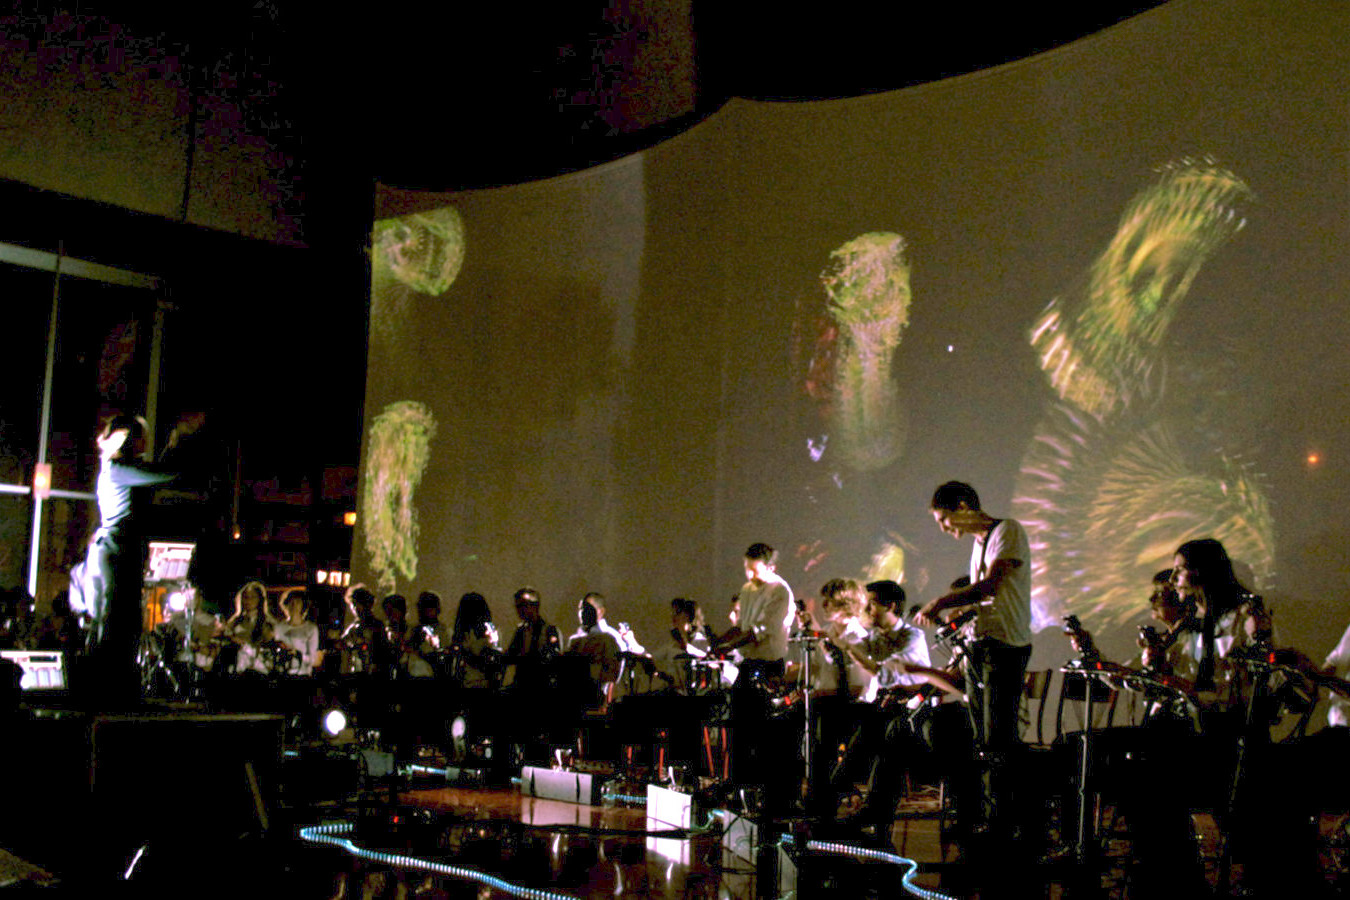
\includegraphics[width=\linewidth]{gfx/02_ephemeral/MetaOrchestre.jpg}
		\caption[Méta-Orchestre, jouant collectivement sur le logiciel Méta-Mallette]{Le Méta-Orchestre de PuceMuse, jouant collectivement sur le logiciel Méta-Mallette. Photographie \copyright Puce Muse.}
		\label{fig:ephemeral:meta-orchestre}
	\end{minipage}
	\hspace{.02\linewidth}
	\begin{minipage}[t]{0.48\textwidth}
	  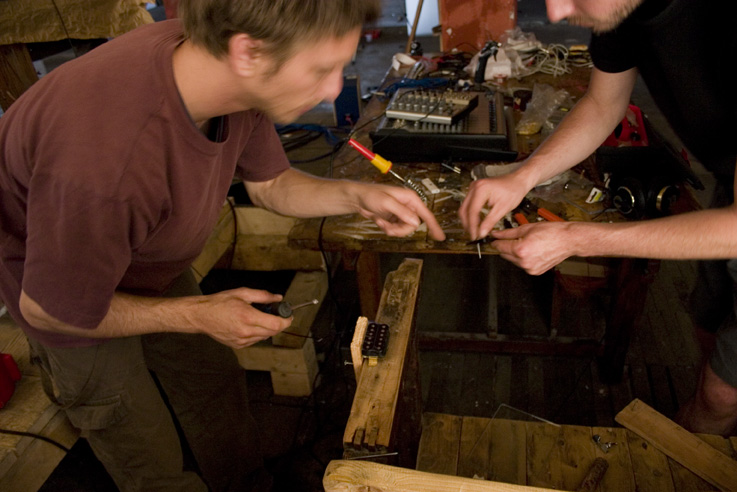
\includegraphics[width=\linewidth]{gfx/02_ephemeral/MediaMusicRoom.jpg}
		\caption[Media Music rooM, transformation collective d'un lieu en instrument de musique]{Media Music rooM, un projet de l'auteur visant à transformer collectivement un lieu en instrument de musique collectif. Photographie : Ivo Ivanov.}
		\label{fig:ephemeral:mediamusicroom}
	\end{minipage}
\end{figure}
%------------------ Figure : collective instruments ---------------------

\subsubsection{DIY-DMI}

\noindent Le \gls{DIY}, en tant qu'approche empirique voire sauvage, est associée au mouvement du \gls{circuit-bending}, consistant à détourner des équipements électroniques à des fins musicales, plutôt qu'à concevoir des instruments de toute pièce. Ce mouvement s'est développé dans les années 1970, en raison de la disponibilité croissante d'appareils électroniques domestiques bon marché et l'inaccessibilité économique des synthétiseurs professionnels, donnant lieu conjointement à une nouvelle esthétique musicale, comme le note Nicolas Collins\footnote{Auteur de l'ouvrage ``Handmade Electronic Music''~\cite{collins_handmade_2006} qui accompagna la seconde vague de \gls{DIY} dans les années 2000.} (cf. Annexe \ref{appendix:collins}): \iquote{(...) there was a kind of a movement in America of homemade and handmade circuitry for music and the reason was that it was primarily economic, which is that the electronic music equipment of the time, synthesizers, were too expensive for a person to buy. (...) But then a kind of a movement started about a kind of an alternative electronic music that was based not so much on using electronic sound to realize an existing vision but as David Tudor called it : ``composing inside electronics''.}\\
\indent Par la suite, l'arrivée au début des années 2000 de micro-contrôleurs facilement programmables et bon marché\footnote{La figure \ref{fig:ephemeral:DIY-devices} témoigne de l'évolution fulgurante de l'accessibilité de ces technologies : l'Eobody, interface d'acquisition de capteurs commercialisée en 2003 pour environ 300€; l'arduino, programmable et offrant des fonctions similaires, commercialisé en 2005 pour quelques dizaines d'euros seulement; le Raspberry Pi commercialisé en 2013 propose pour 35€ un nano-ordinateur de la taille d'un arduino; la plateforme BeagleBone+Bela commercialisée en 2016 permet pour 100€ de disposer d'un nano-ordinateur et une interface audio à latence ultra-faible dans le même facteur de forme.} (cf. figure \ref{fig:ephemeral:DIY-devices}), ainsi que le développement de forums d'échange d'information sur Internet a renouvelé la pratique \gls{DIY}, avec des cartes électroniques telles qu'arduino\footnote{\url{https://www.arduino.cc}}, et des nano-ordinateurs tels que teensy\footnote{\url{https://www.pjrc.com}}, Raspberry Pi\footnote{\url{https://www.raspberrypi.org}}, Bela\footnote{\url{https://www.bela.io}}, etc. Ce second mouvement a également été accompagné par l'émergence de \glspl{makerspace} et de \glspl{fab-lab}.
%------------------ Figure : DIY-LiveCoding ---------------------
\begin{figure}[!htbp]
	\captionsetup{format=plain}%
	\centering
	\begin{minipage}[t]{0.48\textwidth}
		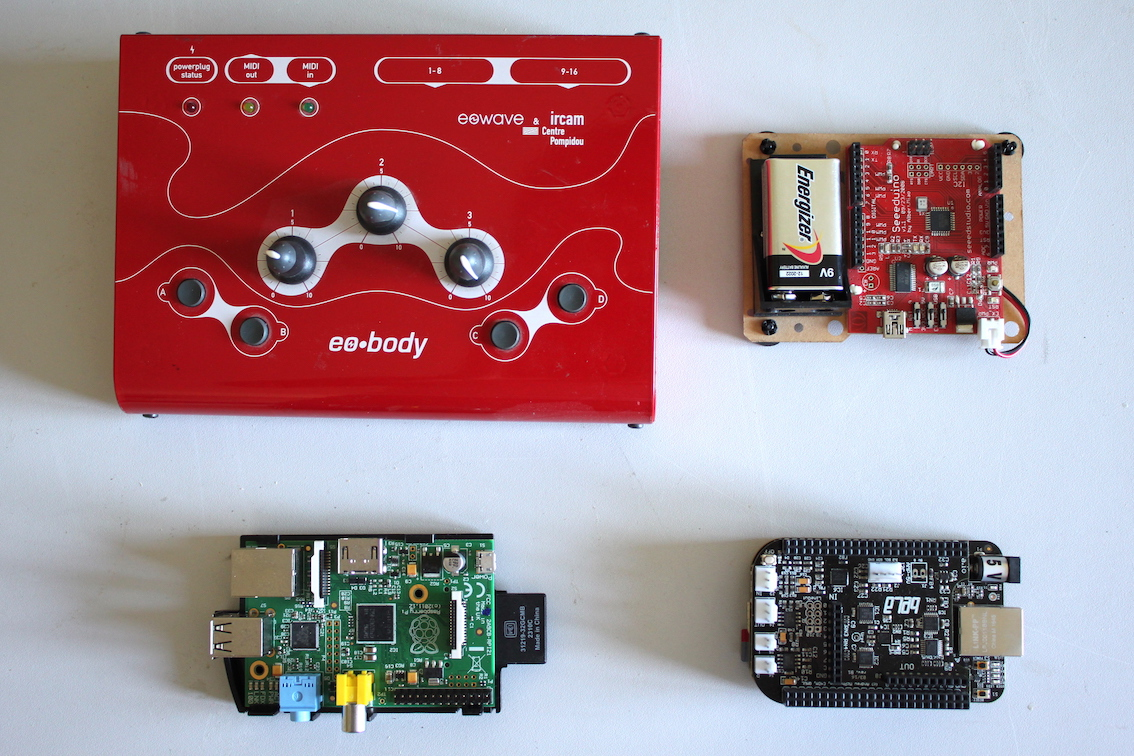
\includegraphics[width=\linewidth]{gfx/02_ephemeral/Eobody-arduino-raspi-bela_144px.jpg}
		\caption[Eobody, Arduino, Raspberry Pi, Bela]{De haut en bas et de gauche à droite: Eobody, Arduino, Raspberry Pi, Bela.}
		\label{fig:ephemeral:DIY-devices}
	\end{minipage}
	\hspace{.02\linewidth}
	\begin{minipage}[t]{0.48\textwidth}
	  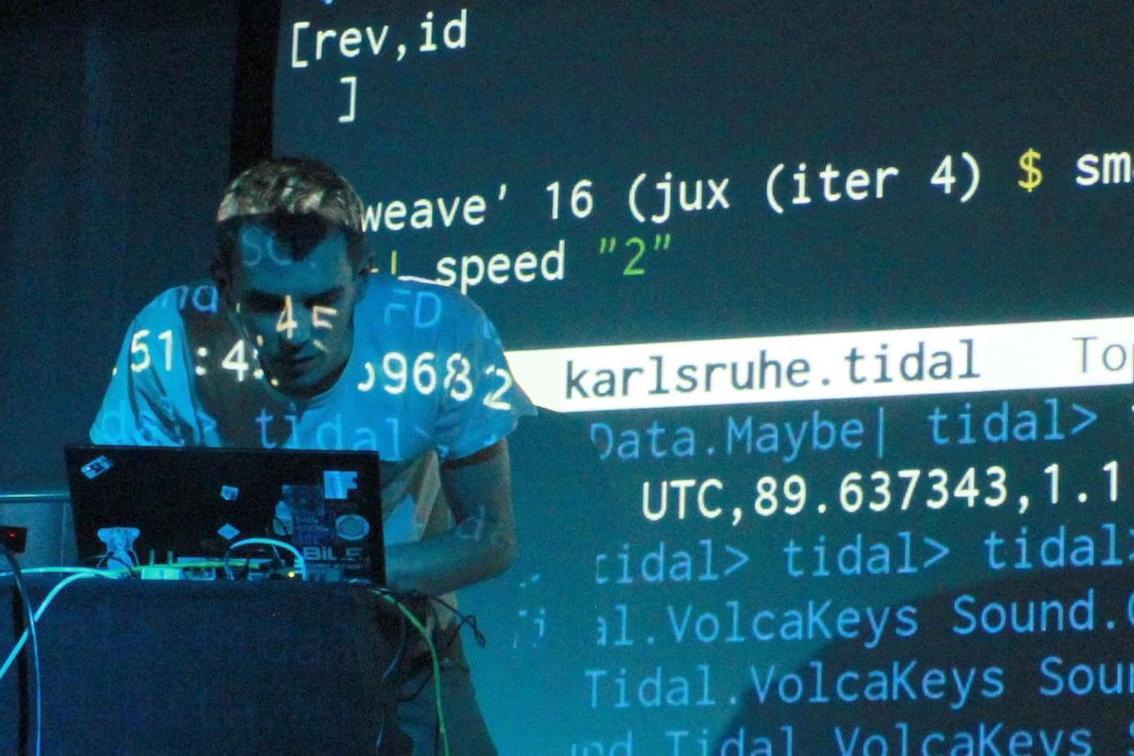
\includegraphics[width=\linewidth]{gfx/02_ephemeral/alex_mclean_144px.jpg}
		\caption[Alex McLean, live-coding avec le langage Tidal Cycles]{Alex McLean, live-coding avec le langage Tidal Cycles.}
		\label{fig:ephemeral:livecoding}
	\end{minipage}
\end{figure}
%------------------ Figure : DIY-LiveCoding ---------------------

%--------------------------------------------------------------
\subsubsection{Live Coding}

\noindent Le \textit{live coding} s'est développé au début des années 2000, comme une pratique visant à créer en direct et de manière semi-improvisée des programmes de création musicale. Cette pratique a été rendue possible par l'orientation de certains logiciels dans une optique de performance live, en particulier SuperCollider \cite{mccartney_rethinking_2002} et le développement dans cette même perspective de logiciels tels que ChucK\footnote{créé à l'université de Princeton par Ge Wang and Perry Cook, voir \cite{wang_chuck_2003}.} en 2003, ou TidalCycles\footnote{créé par Alex McLean, voir \cite{mclean_tidalpattern_2010}, \url{https://tidalcycles.org}.} en 2009, permettant l'interprétation à la volée de code créant et contrôlant des modules de synthèse\footnote{une liste relativement exhaustive de langage de \textit{live coding} est disponible ici : \url{https://github.com/toplap/awesome-livecoding}.}. Ce mouvement s'est également structuré dans une communauté d'échange sur Internet soutenue en particulier par l'association TOPLAP\footnote{\url{https://toplap.org}} et depuis 2015 l'\gls{ICLC}. Le live-coding est une pratique musicale vivante et active, dont le langage de programmation constitue l'instrument \cite{blackwell_programming_2005} et dont l'interface de jeu est souvent le clavier d'ordinateur.\\

%--------------------------------------------------------------

\subsubsection{Installations sonores et instruments à la frontière}

\noindent Enfin, dans la prolifération croissante de systèmes sonores et musicaux qui caractérise ce dernier siècle, les installations sonores interactives constituent une autre forme d'expérience participative du sonore, que celle généralement associée à l'idée d'instrument de musique. A mi-chemin entre la composition, la sculpture et l'instrument, elles ne permettent souvent qu'une pratique éphémère et/ou partielle de la musique (ou simplement du son) donnée à entendre. Elles représentent toutefois un axe révélateur des nouveaux termes dans lesquels la musique et l'instrument s'inscrivent dans la société, en rapprochant les rôles de l'instrumentiste et de l'auditeur, en imbriquant la notion d'instrument et de composition, et en interrogeant la notion de concert et de performance.\\
\indent Ce qu'on appelle généralement ``installation sonore'' conserve toutefois l'idée d'un lieu et d'un moment consacré à l'écoute (ainsi que l'idée d'un artiste auteur), mais l'autonomie propre à l'instrument électrique l'a progressivement entraîné --~depuis un siècle déjà~-- hors des cadres ``concertants'', dans des usages personnels hybrides entre instruments d'écoute et de performance (des bandes magnétiques au web-streaming\footnote{Voir notamment, dans des perspectives différentes d'utilisations musicales du réseau, les projets \textit{WJ-S} d'Anne Roquigny (\url{https://www.wj-s.org}), les mashups Youtube de Kutiman (\url{https://youtu.be/WoHxoz_0ykI}, les sonifications du web du collectif \textit{Art of Failure} \url{http://artoffailure.free.fr/} ou encore les fragments de code audio-génératifs postés sous forme de tweets du projet \textit{sc140} \url{https://twitter.com/sc140tweets}. Pour une réflexion stimulante sur la question des pratiques musicales en réseau, voir notamment \cite{joy_epoque_2009}.}, en passant évidemment par la platine vinyle) qui se prolongent dans la prolifération des \textit{apps}\footnote{Comme l'application RjDj, une des premières ayant souligné cette hybridation sur les smartphones.} audio-musicales sur les ordinateurs mobiles.
%--------------------------------------------------------------
\subsection{Musical organics}
\label{sec:ephemerality:musical-organics}

\noindent On voit que la diversité des lutheries numériques rend leur classification problématique, autant que celle des instruments acoustiques classiques qui se retrouvent augmentés. Pourtant, une telle classification peut être souhaitable, dans la mesure où elle fournit un cadre référentiel d'échange et de discussion entre luthiers, des critères d'analyse pour le musicologue, ainsi que des points de repère pour le compositeur souhaitant travailler avec de tels instruments. \\
\indent Parmi les différentes proposition d'organologie des \glspl{DMI}, celle proposée par Thor Magnusson dans \cite{magnusson_musical_2017} qu'il nomme ``\textit{Musical Organics}''\footnote{L'expression se traduit difficilement en français, ``organics'' renvoyant à l'idée d'organologie autant qu'à l'idée d'organicité, i.e. l'organisation d'un être ``vivant''.} semble particulièrement intéressante en ce qu'elle considère l'organisation des instruments de musique en fonction de l'agencement ``organique'' de leurs éléments.\\
\indent Cette classification propose ainsi d'adopter un modèle rhizomatique, représentant de manière plus adaptée les connexions qui se créent entre différents ``organes'' constitutifs d'un instrument, qu'ils soient \textit{matériaux} (e.g. plastique, métal, verre, etc.), \textit{capteurs} (e.g. \gls{FSR}, microphones, potentiomètres, etc.), \textit{sons} (e.g. échantillons, synthèse FM, additive, etc.), \textit{\glspl{mapping}} (e.g. fonctions de transfert, apprentissage, stochastique, etc.), \textit{gestes} (e.g. frapper, pincer, frotter, etc.), ou tout autre aspect culturel, technique, musicologique ou appartenant à un quelconque domaine entretenant un lien avec la lutherie.\\
\indent Magnusson note que cette organisation, au-delà de l'aspect descriptif déjà présent dans les organologies traditionnelles, devrait se prêter à une \iquote{organologie interprétative, qui pose les questions du `pourquoi' et du `comment', et offre des explications en replaçant ces questions dans leurs contextes historiques et musicologiques.}

%%%%%%%%%%%%%%%%%%%%%%%%%%%%%%%%%%%%%%%%%%%%%%%%%%%%%%%%%%%%%%%
\section{Une critique de la longévité}
\label{sec:ephemerality:critique}

\noindent Ce foisonnement dans le paysage des \gls{DMI} et la difficulté à établir des catégories qui se raccordent avec les classifications classiques coïncident avec une question plus générale portant sur la longévité de ces instruments. En effet, comment établir des catégories si les objets que l'on souhaite classer sont en mutation permanente ? Et comment partager, transmettre, enseigner, pratiquer la musique avec des objets aussi instables ?

\subsection{DMI will survive}

\noindent La longévité des \glspl{DMI} est une question complexe qui a été soulevée à plusieurs reprises dans la littérature des \gls{NIME} (et d'autres domaines connexes) et fait l'objet d'un débat croissant au cours de la dernière décennie \cite{baguyos_contemporary_2014, morreale_design_2017,bonardi_preservation_2008}. Les auteurs qui se sont intéressés à cette question ont identifié un certain nombre de causes de cette situation, qu'elles soient techniques, méthodologiques ou sociologiques, et ont apporté réflexions et propositions pour y remédier, telles que de nouveaux environnements pour concevoir et évaluer les instruments \cite{jorda_digital_2004, morreale_design_2017}, une meilleure documentation, de nouvelles méthodes pédagogiques et la création de communautés, ainsi qu'un travail visant à établir une notation musicale et un répertoire pour ces nouveaux instruments \cite{mamedes_composing_2014,mays_notation_2014}. Cependant, dans la majorité de ces articles, le manque de longévité des \glspl{DMI} est essentiellement considéré comme un défaut, ou du moins un problème à résoudre.\\
\indent Dès 1975, des compositeurs de musique électroacoustique au \gls{GRM} réfléchissaient aux questions de préservation soulevées par une musique \iquote{écrite sur du sable}\footnote{Michel Chion emploie cette formule dans \cite{chion_musique_1977}, en faisant référence aux particules ferro-magnétiques des bandes audio, vouées à une dégradation prochaine.} : certains compositeurs disaient qu'ils s'en moquaient et faisaient leur musique pour le présent, tandis que d'autres voyaient dans l'ère numérique naissante la possibilité de préserver leurs œuvres dans le futur. Comme nous le savons aujourd'hui, troquer le sable contre le silicium (ou le nuage, maintenant) n'a pas totalement résolu le problème.\\
\indent Les \glspl{DMI} ayant largement intégré la partie compositionnelle des œuvres musicales, parfois même confondue avec l'instrument, le désir de préserver les œuvres musicales s'est trouvé partiellement transposé dans la question de la conservation des instruments et des outils utilisés pour leur production. Mais quelles sont les raisons de cette quête de longévité ? Et qu’est-ce qui légitime à ce point la longévité d’un instrument pour qu’elle soit d’emblée vue comme une qualité ? 

\indent Le désir de longévité est lié ontologiquement à une réaction profondément enracinée dans notre condition de simples mortels, qui consiste à chercher un moyen d'assurer notre survie, notamment par la transmission des connaissances et la création de traditions. Le paléoanthroplogue André Leroi-Gourhan a analysé le phénomène des traditions comme un moyen d'extérioriser et de transmettre notre mémoire à travers la création de systèmes techniques et de ``chaînes opératoires'' \cite{leroi-gourhan_geste_1964}. Plus récemment, Bernard Stiegler s'est appuyé sur cette idée pour définir le concept de ``grammatisation'', comme processus par lequel le \textit{continuum} temporel des comportements humains est transformé en un spatial discret, ce qui permet de les intégrer dans des outils \cite{stiegler_for_2010}.\\
\indent Les humains ont ainsi développé des méthodes et des outils, tels que la psalmodie de textes (surtout religieux) ou l'écriture comme moyens à la fois d'enregistrer des informations pour un usage ultérieur et de transmettre des connaissances à ceux qui y survivent. L'écriture a partiellement libéré les humains du besoin de tradition orale en transférant ces connaissances sur un support physique, ce qui lui a également permis de capitaliser et de spéculer sur ses connaissances.\\
\indent Ainsi, la notion de longévité traverse le champ des arts et des sciences, aux frontières desquels se trouvent les instruments de musique. Dans l'histoire de l'art, il reste principalement les œuvres durables, ``gravées dans le marbre'', dont sont faites les sculptures. De même, la science aspire à trouver des lois durables pour décrire le monde observable et les formuler dans le langage pérenne des mathématiques. Mais si la longévité évidente d'une œuvre constitue souvent un atout pour sa propre légitimation, lorsqu'il s'agit d'un instrument numérique et plus encore lorsqu'il est conçu comme un moyen interactif de créer une expérience musicale par essence éphémère, la question ne semble pas pouvoir se régler dans les mêmes termes.\\

	
\subsection{Longevité, adoption, succès}

\noindent Deux aspects semblent être souvent confondus : la longévité d'un instrument d'une part et son ``succès'' d'autre part. De plus, la notion de succès, éminemment sujette à la perspective adoptée, semble être souvent considérée comme le taux d'adoption par une communauté d'instrumentistes, au-delà des aspects financiers d'un succès commercial.\\
\indent Ces trois aspects, longévité, succès et adoption, sont cependant relativement différents, en partie indépendants et parfois même contradictoires. Il existe des exemples notoires de ce décalage: \textit{The Hands} de Michel Waisvisz \cite{torre_hands:_2016} (Figure \ref{fig:ephemeral:Waisvisz_TheHands}), le \textit{Lady's Glove} de Laetitia Sonami \cite{sonami_my_2006} (Figure \ref{fig:ephemeral:Sonami_LadysGlove}) ou encore le \textit{Méta-Instrument} de Serge De Laubier \cite{couprie_meta-instrument:_2018} (Figure \ref{fig:ephemeral:DeLaubier_MI4}) sont trois instruments ayant eu une longévité remarquable\footnote{Plus de 20 ans pour \textit{The Hands} --~jusqu'au décès de Michel Waisvisz, 28 ans pour le \textit{Lady's Glove} et plus de 30 ans pour le \textit{Méta-Instrument} dont l'actuelle 4\textsuperscript{e} version a été finalisée en 2019.}, soutenue par une pratique régulière de leur inventeurs, sans toutefois avoir été adopté par une large communauté d'instrumentistes. Inversement, l'éphémérité d'un outil ne mène pas systématiquement à une absence de popularité\footnote{Considérons ici tous les gadgets éphémères qui, sous l'influence d'une mode et/ou d'une puissante campagne publicitaire, envahissent le marché, ou encore tous les appareils qui deviennent obsolètes lorsqu'un nouvel appareil les remplace, tels que le smartphone qui, outre le remplacement de nos anciens téléphones, a également balayé d'un coup les lecteurs mp3, les GPS, les consoles de jeux portables, les lampes de poche, les montres, etc.} et encore moins à un manque d'intérêt musical pour les performances réalisées avec ces instruments.\\
%------------------ Figure : Waisvisz — De Laubier ---------------------
\begin{figure}[!htbp]
	\captionsetup{format=plain}%
	\makebox[\linewidth][c]{%
		\begin{subfigure}[b]{.35\textwidth}
			\centering
			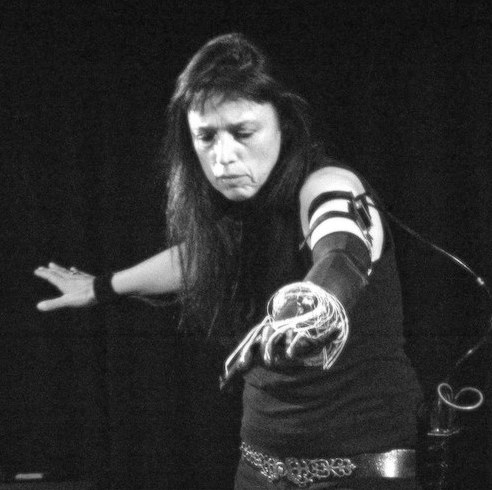
\includegraphics[width=.98\textwidth]{gfx/02_ephemeral/Sonami.jpg}
			\caption[Laetitia Sonami et le Lady's Glove]{L. Sonami: Lady's Glove\\ photographie: Charles Kremenak}
			\label{fig:ephemeral:Sonami_LadysGlove}
		\end{subfigure}%
		\begin{subfigure}[b]{.35\textwidth}
			\centering
			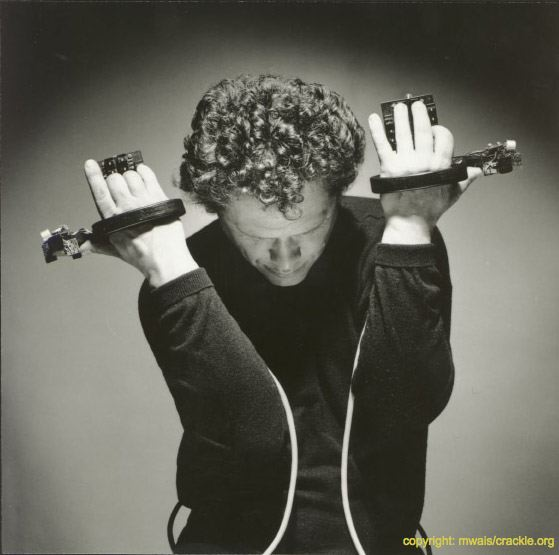
\includegraphics[width=.98\textwidth]{gfx/02_ephemeral/Waisvisz_TheHands.jpg}
			\caption[Michel Waisvisz et The Hands v2]{M. Waisvisz: The Hands\\ photographie: Carla van Thijn}
			\label{fig:ephemeral:Waisvisz_TheHands}
		\end{subfigure}%
		\begin{subfigure}[b]{.35\textwidth}
			\centering
			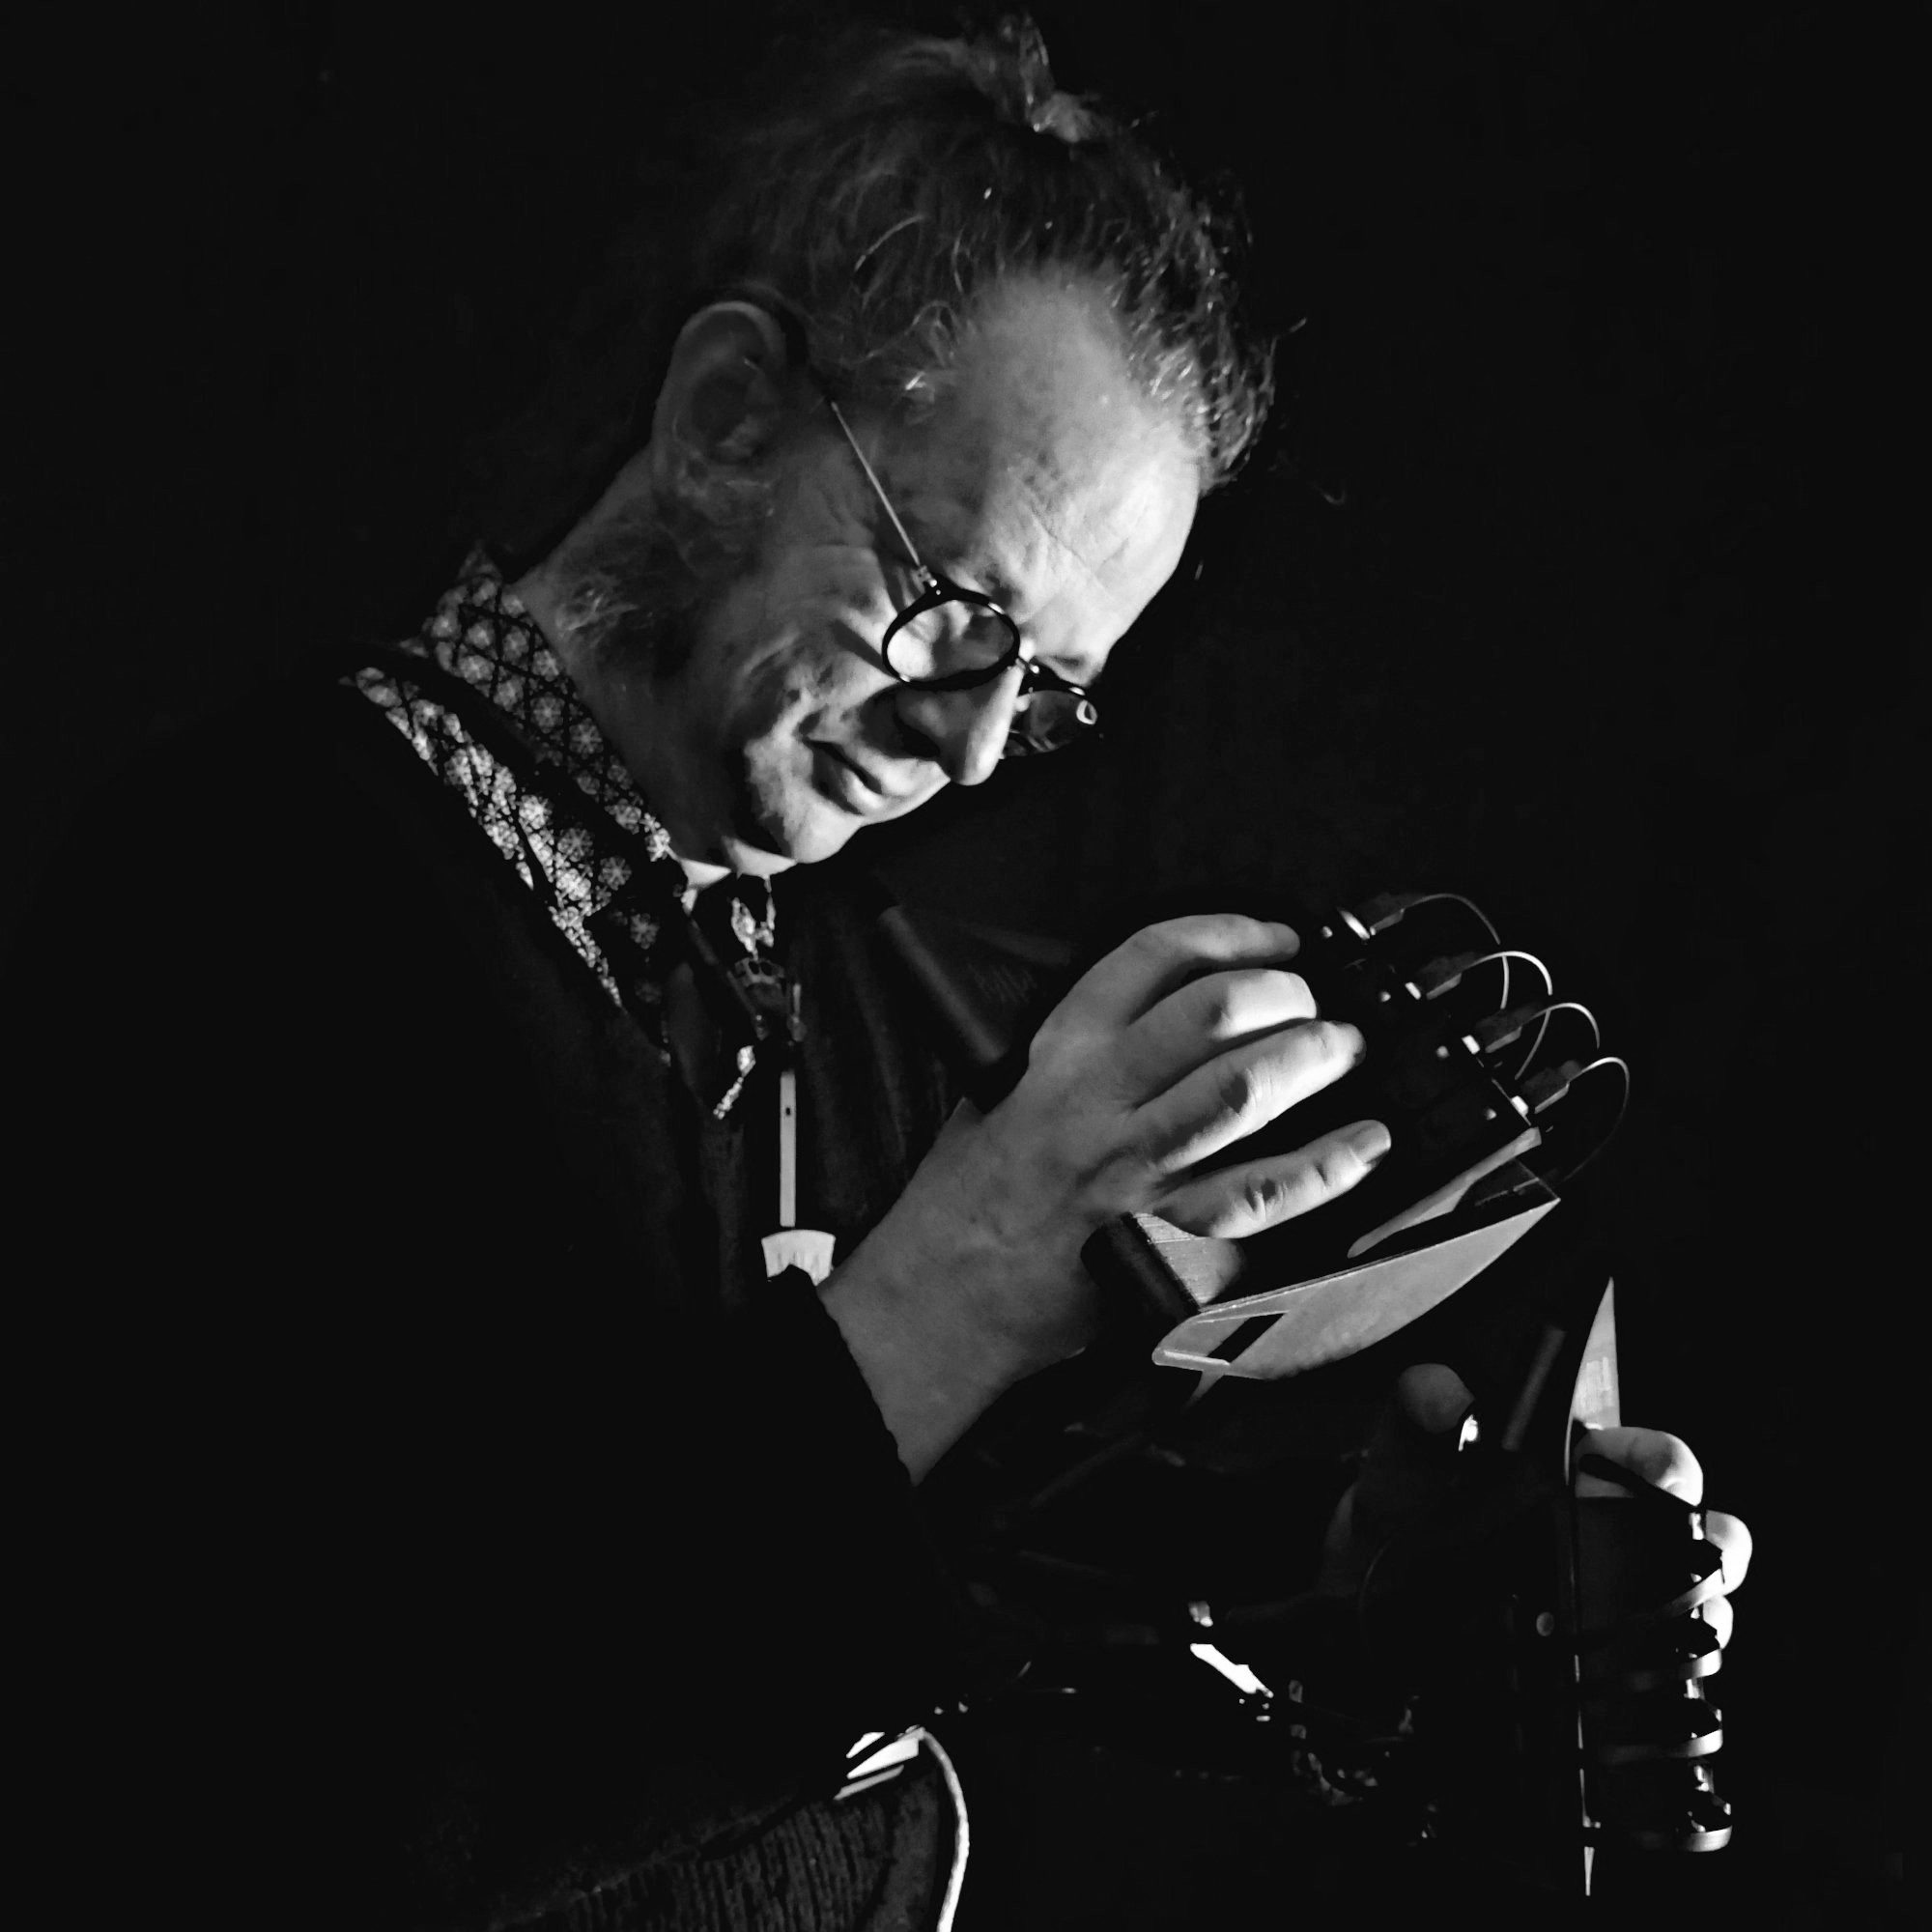
\includegraphics[width=.98\textwidth]{gfx/02_ephemeral/DeLaubier-MI4.jpg}
			\caption[Serge de Laubier et le Méta-Instrument 4]{S. de Laubier: Méta-Instrument\\ photographie: Puce Muse}
			\label{fig:ephemeral:DeLaubier_MI4}
		\end{subfigure}%
	}
	\caption[Lady's Glove, The Hands, Méta-Instrument: durabilité n'est pas synonyme d'adoption]{\textit{Lady's Glove}, \textit{The Hands}, \textit{Méta-Instrument}: durabilité n'est pas synonyme d'adoption par un large public.}
\end{figure}
%------------------ Figure : Waisvisz — De Laubier ---------------------
\indent La notion de succès dépend ainsi de la perspective adoptée, selon qu'elle soit celle des luthiers qui créent des instruments pour d'autres ou de ceux qui créent des instruments pour eux-mêmes\footnote{L'étude de Morreale et McPherson \cite{morreale_design_2017} tend à montrer une majorité des seconds dans les participants à la conférence \gls{NIME}}. Dans ce dernier cas, l'adaptation de l'instrument aux besoins ou à l'esthétique propres de l'instrumentiste peut s'avérer telle qu'il soit difficile pour les autres de l'adopter.\\
\indent Également, les évolutions techniques ainsi que les modes peuvent amener à la réapparition d'instruments tombés dans l'oubli. On appréciera ici la perspicacité de François-Alexandre Garsault, cité par Malou Haine \cite{haine_les_2018}, qui dans sa ``Division des instruments selon leurs différentes utilisations'' (1761) classait une série d'instruments, dont la harpe et la ``guitare'' (sic), dans la catégorie des \iquote{Instruments hors d'usage, mais qui peuvent revenir}.


\subsection{Longevité versus stabilité}
\label{sec:ephemeral:longevity_stability}

\noindent La question de la durabilité d'un instrument soulève implicitement la question de sa stabilité historique. Ainsi, l'histoire organologique des instruments de musique européens révèle de nombreux facteurs qui conduisent à l'apparition, à l'évolution ou à la disparition des instruments de musique. À cet égard, les nombreuses innovations technologiques de la révolution industrielle s'avèrent intéressantes car cette période bien documentée illustre les débuts des grandes révolutions qui allaient se produire au \siecle{20}~siècle, tout en soulevant la question même de la stabilité de la forme des instruments. Ainsi, lorsque le traverso fut équipé du système de clétage inventé par Théobald Boehm en 1832 et devint une flûte traversière, s'agissait-il d'un nouvel instrument ? À quel moment décidons-nous qu'un instrument qui subit des changements n'est plus le même ?

\subsection{Éphémérité dans le contexte musical}
\label{sec:ephemeral:ephemerality_in_musical_context}

\subsubsection{Impermanence du phénomène sonore}
\noindent Rappelons tout d'abord une évidence : la musique elle-même est intrinsèquement intangible, évanescente et nécessite une énergie entretenue pour exister : le phénomène sonore est en éphémérité permanente. La musique, dans sa forme sensible, n'existe que pendant le temps de sa performance. Bien que les instruments utilisés pour la produire puissent être durables, leur convocation et le son lui-même sont toujours temporaires\footnote{À tel point que les pièces qui mettent au défi cette éphémérité, telles que les \textit{Vexations} d'Erik Satie ou encore \textit{Organ²/ASLSP} de John Cage sont des exceptions notoires.}.

\subsubsection{De la performance}

\noindent Même lorsqu'elle est notée sur une partition, la musique en tant qu'art vivant est en constante réinterprétation. Cette interprétation permet de transformer une partition notée sous forme symbolique en une expression sensible sujette à variations. On peut objecter que cette interprétation n'existe que lorsque la musique est notée de manière symbolique, laissant aux interprètes la possibilité de la jouer à leur façon dans le contexte de l'interprétation. Mais est-ce toujours le cas lorsque la musique est `intégralement notée' jusqu'au son lui-même, comme c'est le cas sur un disque audio ? Cela signifie-t-il que l'interprétation disparaît ? Les performances de spatialisation en direct de la musique électroacoustique par des musiciens professionnels ou les différentes pratiques de remixes que l'on retrouve dans le hip-hop tendent à prouver le contraire. Toute performance musicale, même la simple écoute d'un disque, convoque inévitablement un nouveau contexte d'écoute, car elle se produit nécessairement dans un moment présent unique. Entre le son enregistré et son écoute, on retrouve la même \textit{différance}\footnote{La \textit{Différance} est un concept proposé par Derrida \cite{derrida_lecriture_2014} pour désigner à la fois l'ajournement (le fait de différer) et la différenciation qui se créé entre un texte et sa signification.} qu'entre une partition et ses interprétations.

\subsubsection{Une esthétique musicale mûe par le mouvement}

\noindent Par ailleurs, la musique contemporaine occidentale poursuit une quête de la nouveauté et de territoires sonores inexplorés, comme le soulignait Jean-Claude Risset dans son discours invité à Athènes en 2014 : \iquote{(...) la musique contemporaine met en évidence ce qui a été rejeté dans le monde grec : elle capte davantage l'évanescent, l'éphémère, l'ambivalent, l'Erebus, elle favorise la métamorphose sans fin des qualités et des formes; comme Nietzsche l'a déclaré, la musique occidentale tend vers la libération de la dimension dyonisiaque et l'acceptation du côté inacceptable des mythes}\footnote{\iquote{[Hugues] Dufourt suggest that contemporary music highlights what was rejected in the Greek world : it rather captures the evanescent, the ephemeral, the ambivalent, the Erebus, it favors the endless metamorphosis of qualities and forms; as Nietzsche proclaimed, western music tends toward the liberation of the dyonisiac dimension and the acceptance of the inacceptable part of myths.} \cite{risset_sound_2014}}.\\
%\indent Cette d'attraction pour l'éphémère et la métamorphose s'est traduite dans la recherche permanente de nouveaux modes de jeu et de nouveaux timbres de la part de l'instrumentiste et du compositeur, mais surgit également dans le travail du luthier à mesure que son outil de travail gagne une souplesse qui le rapproche de la souplesse gestuelle de l'instrumentiste ou de celle de la pensée du compositeur.


\subsubsection{Partitions dynamiques, ouvertes, ad-hoc}
\label{sec:ephemeral:longevity_stability:dynamic_scores}

\noindent Les partitions musicales sont en partie intégrées dans les \glspl{DMI}, pour lesquels Norbert Schnell et Marc Battier ont proposé le terme ``d'instruments composés'' dans \cite{schnell_introducing_2002}\footnote{L'idée d'instruments composés est toutefois plus ancienne, voir Harry Partch ou Gordon Mumma (1967) : \iquote{My own electronic music equipment is designed as part of the process of composing my music. I am really like the composer who builds his own instruments, though most of my ``instruments'' are inseparable from the compositions themselves.}\cite{mumma_creative_1967}}. La partition elle-même a fait l'objet d'une reconfiguration plus ouverte depuis le milieu du \siecle{20}~siècle et les compositeurs ont progressivement intégré les possibilités algorithmiques dans leurs processus de création : des systèmes dynamiques et interactifs mettent en mouvement la stabilité des figures de notes. Plusieurs compositeurs\footnote{Parmi ceux qui ont écrit et analysé des partitions dynamiques, voir les œuvres de Hajdu \cite{hajdu_disposable_2016}, Bhagwati \cite{bhagwati_vexations_2017} ou Freeman \cite{freeman_extreme_2008}.} questionnent ainsi la stabilité de la partition en utilisant l'ordinateur pour créer des instances \textit{ad hoc}, soit à l'aide d'algorithmes génératifs, soit en introduisant des parties improvisées dans des formes hybrides pour lesquelles Richard Dudas propose le terme de ``comprovisation'' \cite{dudas_comprovisation:_2010}. Se pourrait-il que la technologie numérique offre ce support idéal permettant à la fois la préservation des œuvres musicales en même temps que leur mutation ?

\subsubsection{Obsolescence de la technologie}

\noindent Les matériaux utilisés pour les instruments acoustiques semblent vieillir relativement bien. Le matériel électronique vieillit mal en comparaison et le cuivre de ses circuits est plus fragile que celui des trompettes, saxophones et autres cuivres. Par ailleurs, la miniaturisation extrême des microprocesseurs les rend généralement impossibles à réparer ; ils sont souvent remplacés par de nouvelles versions possiblement incompatibles. Le code informatique, dans sa forme compilée, est tout aussi cryptique que le microprocesseur : un bloc illisible qui incarne le paradoxe de la notation informatisée par rapport au papier traditionnel - ``nous écrivons des choses que nous ne pouvons plus relire''\footnote{Kevin Slavin dans la conférence ``Comment les algorithmes façonnent notre monde'', \url{https://www.ted.com/talks/kevin_slavin_how_algorithms_shape_our_world}}. Et quand le système d'exploitation sera mis à jour, il y a des chances qu'il ne pourra plus les lire non plus.\\
\indent Dans un article où il compare les différences ontologiques entre \textit{hardware} et \textit{software}, Nicolas Collins \cite{collins_semiconducting_2013} résume leur relation au temps avec la formule : \iquote{hardware is yesterday, software is now}, ce qui pourrait se traduire par le fait que le logiciel est en permanence mis à jour tandis que le hardware est toujours dépassé. Ni l'un ni l'autre ne semble être en mesure d'offrir une continuité fiable entre le passé et l'avenir.

	
\subsubsection{Économie de la nouveauté}

\noindent A l'obsolescence de la technologie, s'ajoutent les effets de la société de consommation. Depuis plus d'un siècle, l'industrie fait de plus en plus la promotion d'un paradigme jetable en encourageant les consommateurs à \iquote{acheter pour le style, pas seulement pour les améliorations technologiques} \cite{slade_made_2006} et en organisant une obsolescence programmée.\\
\indent Ce modèle économique a également affecté celui des arts du spectacle, qui promeut la création bien plus que la reprise d'un spectacle à tel point que, comme le rappelle Georg Hajdu dans \cite{hajdu_disposable_2016} : \iquote{Les pièces connaissent rarement plus qu'une seule représentation}. De même, les résidences d'artistes sont plus souvent destinées à de nouvelles créations davantage qu'à la poursuite d'œuvres antérieures.\\
\indent Cette économie de l'obsolescence (planifiée ou non) ne favorise pas l'attachement à un instrument et, en ce qui concerne les contrôleurs MIDI commerciaux, le plastique bon marché dont ils sont le plus souvent faits dégrade la valeur qui peut être attribuée à un instrument acoustique traditionnel. L'attachement et l'engagement avec les instruments virtuels sont également remis en question par leur nature immatérielle. La plupart des logiciels commerciaux s'orientent maintenant vers une économie basée sur l'abonnement plutôt que sur l'achat, puisque l'achat ne garantit plus ni la durabilité ni la propriété de l'objet.

	
\subsubsection{L'instrument comme compromis instable}

\noindent L'instrument de musique est aussi, comme le souligne Bernard Sève dans \cite{seve_instrument_2013} : \iquote{un compromis instable entre des qualités non-convergentes}. Pour les instruments acoustiques, ce compromis entre ergonomie gestuelle et performance acoustique, imposé par la physicalité des matériaux, est généralement fixé dans un assemblage ajusté et collé. Ce montage agit comme un facteur de stabilisation par rapport à un environnement numérique dans lequel l'absence de contraintes physiques laisse l'instrument à cœur ouvert, prêt à être modifié à tout instant.\\
\indent Bill Buxton soulignait la différence entre les spécifications standard, militaires et artistiques pour souligner l'exigence plus élevée de cette dernière \cite{buxton_artists_1997}. Le design des objets d'art exige une grande finesse, en effet. Accorder les qualités sonores et ergodynamiques\footnote{Thor Magnusson a proposé ce terme dans \cite{magnusson_ergodynamics_2019} pour nommer le \iquote{pouvoir et la profondeur expressive d'un instrument}.} d'un instrument de musique s'apparente à la quête d'un \textit{inframince}\footnote{\label{fn:inframince}Marcel Duchamp \cite{duchamp_notes_2008} a inventé le terme \textit{inframince} dans une série d'exemples décrivant une différence si infime qu'elle ne peut être qu'imaginée, par exemple \iquote{La différence entre deux objets faits en série (sortis du même moule) est un inframince quand le maximum de précision est obtenu.}} pour lequel il n'existe pas de spécifications convenues. Cependant, une autre particularité des technologies utilisées pour les performances live est qu'elles sont \iquote{dévolues à une expérience, pas à une bande-son, inutiles pour la relecture, la sauvegarde, l'échange ou la duplication}, comme le note Nicolas Collins dans \cite{collins_semiconducting_2013}.\\
\indent Ainsi, la pérennité de l'instrument en dehors de la durée même de la performance n'est pas un critère essentiel et il n'est pas rare que les musiciens numériques\footnote{Andrew Hugill définit un \textit{musicien numérique} dans \cite{hugill_digital_2019} comme \iquote{quelqu'un qui a saisi les possibilités ouvertes par les nouvelles technologies, en particulier le potentiel de l'ordinateur pour explorer, stocker, manipuler et traiter le son, ainsi que le développement de nombreux autres outils et dispositifs numériques qui permettent l'invention et la découverte musicale} soulignant le fait qu'ils sont \iquote{non pas définis par leur seule utilisation de la technologie}, mais ont aussi \iquote{une certaine curiosité, un questionnement et un engagement critique sur ce terrain}.} modifient leur instrument quelques minutes avant le début d'un concert, juste pour les besoins du moment présent.

	
\subsubsection{Esthétique du dysfonctionnement}

\noindent En effet, le risque de dysfonctionnement n'est pas rédhibitoire à de nombreuses performances musicales. Les bugs et artefacts causés par les dysfonctionnements s'avèrent être des sources fertiles de matériaux musicaux et la subversion du fonctionnement cryptique des processeurs en révèle un aspect invisible, faisant ressurgir la nature même du matériau électronique, au-delà de l'objectif pour lequel ils ont été conçus\footnote{Parmi les exemples significatifs, les travaux de Yasuano Tone pour ``Wounded CD'', ceux de Nicolas Collins sur circuits électroniques morts ou encore la sonification de données brutes par Carsten Nicolai illustrent clairement cette approche.}. David Zicarelli\footnote{Zicarelli est le fondateur de \textit{Cycling'74}, entreprise développant et commercialisant le logiciel Max.} le résumait en ces termes : \iquote{Je remarque simplement que dans la plupart des concerts pointus, l'échec a tendance à être beaucoup plus intéressant pour le public que le succès.}\footnote{\iquote{I would only observe that in most high- profile gigs, failure tends to be far more interesting to the audience than success.} cité par Cascone dans \cite{cascone_aesthetics_2000}.}
On peut lire dans cette remarque une tendance essentielle de l'époque post-moderne, caractérisée par un art qui attribue davantage de valeur à \textit{l'intérêt} du geste pris dans un contexte \textit{expérimental}, qu'à sa \textit{qualité}, pris dans un contexte \textit{normatif} classique.

\subsubsection{Plus besoin de tradition?}

\noindent L’apparition de la notation musicale ne rend plus nécessaire la performance à seules fins de transmission, l’enregistrement audio ne rend plus nécessaire la performance à seules fins d’écoute, l’existence de banques de sons ne rend plus nécessaire l’apprentissage d’un instrument particulier pour produire le son de cet instrument\footnote{Voir par exemple, le rendu du Sacre du Printemps d'Igor Stravinsky par Jay Bacal avec la Vienna Sound Library (VSL): \url{https://youtu.be/PB3njyDW8SY.}} et maintenant l’intelligence artificielle rend superflu l'acte même de composition en laissant la possibilité de générer automatiquement des morceaux inédits\footnote{Voir par exemple les productions du projet FlowMachines par François Pachet et al. in \cite{hadjeres_deepbach:_2016}: “Daddy's car” (\url{https://youtu.be/LSHZ_b05W7o}) ou “DeepBach” (\url{https://youtu.be/QiBM7-5hA6o}). L'originalité de ces compositions par \textit{IA}, techniquement basées sur l'imitation d'un corpus existant, reste cependant une question ouverte.}.\\
\indent En 1964, André Leroi-Gourhan, qui voyait dans la machine informatique la possibilité sans précédent d'externaliser la mémoire, se demandait alors ce qui adviendrait si les machines devenaient capables \iquote{[d’écrire] des pièces de théâtre parfaites, [de peindre] des tableaux inimitables} \cite{leroi-gourhan_geste_1964}. En 1992, John Cage semblait lui répondre de façon radicale : \iquote{Nous n'avons pas besoin d'avoir des traditions si nous nous libérons de la mémoire.} \cite{sebestik_ecoute_1992}\\
\indent Cependant, s'il est possible d'évoluer, comme le décrit la philosophe Christine Buci-Glucksmann dans \cite{buci-glucksmann_esthetique_2003}, d'une culture de l'objet à une culture des flux, elle remarque que dans un pays comme le Japon qui valorise positivement l'impermanence, l'éphémère a une place centrale tout en étant profondément ancré dans la tradition.\\
\indent La résolution de cet antagonisme apparent entre la position de Cage et celle de Buci-Glucksmann semble se situer dans le déplacement des objets (ou des flux, en l'occurence) soutenus par la tradition, dans la reformulation des motivations de la pérennité et de l'éphémérité. Davantage que ses calcifications stables, c'est l'étude des dynamiques à l'œuvre dans la création musicale qui pourra nous renseigner sur la manière dont s'agencent les instruments: nous risquons sinon de n'avoir que ``découpé une tranche d'histoire''\footnote{Jean During livre cet avertissement en introduction de \cite{during_quelque_1994} : \iquote{De nos jours où s'accumulent les traces tangibles des musiques passées, il faut donc renoncer à nos illusions : on n'appréhende que du changement, du mouvant, de l'instable. On croyait avoir saisi le fond stable, la structure, l'essentiel, les archétypes, mais on avait simplement découpé une tranche d'histoire.}}.

\section{Articulation du pérenne et de l'éphémère}

\subsection{Les DMI comme agencements instables et sauvages}

\noindent Le terme même de \gls{DMI}, qui a progressivement envahi la littérature des \gls{NIME}, pourrait nous laisser penser qu'il s'agit d'une catégorie bien définie alors qu'il s'agit en fait d'un méli-mélo d'objets qui n'ont de commun que leur utilisation de la computation numérique. Le biais qui en résulte dans l'évaluation de l'incapacité des \glspl{DMI} à atteindre une maturité provient du fait qu'un instrument de musique est encore souvent considéré comme un tout cohérent, devant faire preuve de longévité, à l’image des instruments acoustiques pris comme modèles.\\
\indent Pourtant, la modularité induite par l'électronique et la technologie numérique a ``atomisé'' l'intégrité de l'instrument. Cette atomisation peut être entendue à la fois dans le sens de ``détruit'' mais aussi dans le sens de ``fragmenté en éléments atomiques''. Sur scène, on constate en outre que les \glspl{DMI} s'apparentent souvent à des assemblages prototypiques fragiles\footnote{Pour une réflexion poursuivant à dessein la fragilité —et la destructibilité— des \glspl{DMI}, voir aussi \cite{berthaut_wubbles:_2014, haddad_fragile_2017}.} (cf. Figure \ref{fig:ephemeral:Gordeff}), pleins de câbles (physiques ou virtuels) prêts à être intervertis quelques minutes avant le concert, ou même pendant celui-ci. Pourquoi dans ce cas les envisager comme des monolithes durables plutôt que comme les agencements\footnote{Adoptant ici le concept de Deleuze et Guattari proposé dans \cite{deleuze_mille_1980}; voir aussi ``musical instruments as assemblage'' de Paul Theberge dans \cite{bovermann_musical_2017}.} éphémères qu’ils sont le plus souvent?\\
%\todo{évoquer la notion de behavioural objects de \cite{bown_understanding_2009}}
\indent De ce point de vue, le format académique d'une conférence telle que \gls{NIME} rend difficile la présentation des \gls{DMI} dans leur forme chaotique et leur sélection est biaisée par le fait que leurs auteurs appartiennent souvent au monde académique. Cela favorise la démonstration de critères techniques dûment réfléchis plutôt que la présentation d'un fatras de circuits et d'algorithmes connectés empiriquement et dont on ne comprend rien au fonctionnement, sinon que le musicien qui en joue fait des merveilles.\\
\indent En se confrontant à un agencement instrumental éphémère, l'instrumentiste, tout virtuose qu'il soit, se retrouve nécessairement en tension avec un instrument ``sauvage'' qu'il faut apprivoiser. Cela demande une attention gestuelle et auditive intense et la recherche de résonance avec l'instrument. (Sinon, autant composer tranquillement chez soi et fournir à l’auditeur un support sur lequel il n’aura qu’à appuyer sur la touche \textit{play}). Peut-être davantage que la longévité, on pourra y voir un critère de lutherie intéressant : la possibilité que l'instrument dérape et devienne hors de contrôle.

%-------------------------- Figure : Gordeff ----------------------------------
\begin{figure}[!htbp]
	\captionsetup{format=plain}%
	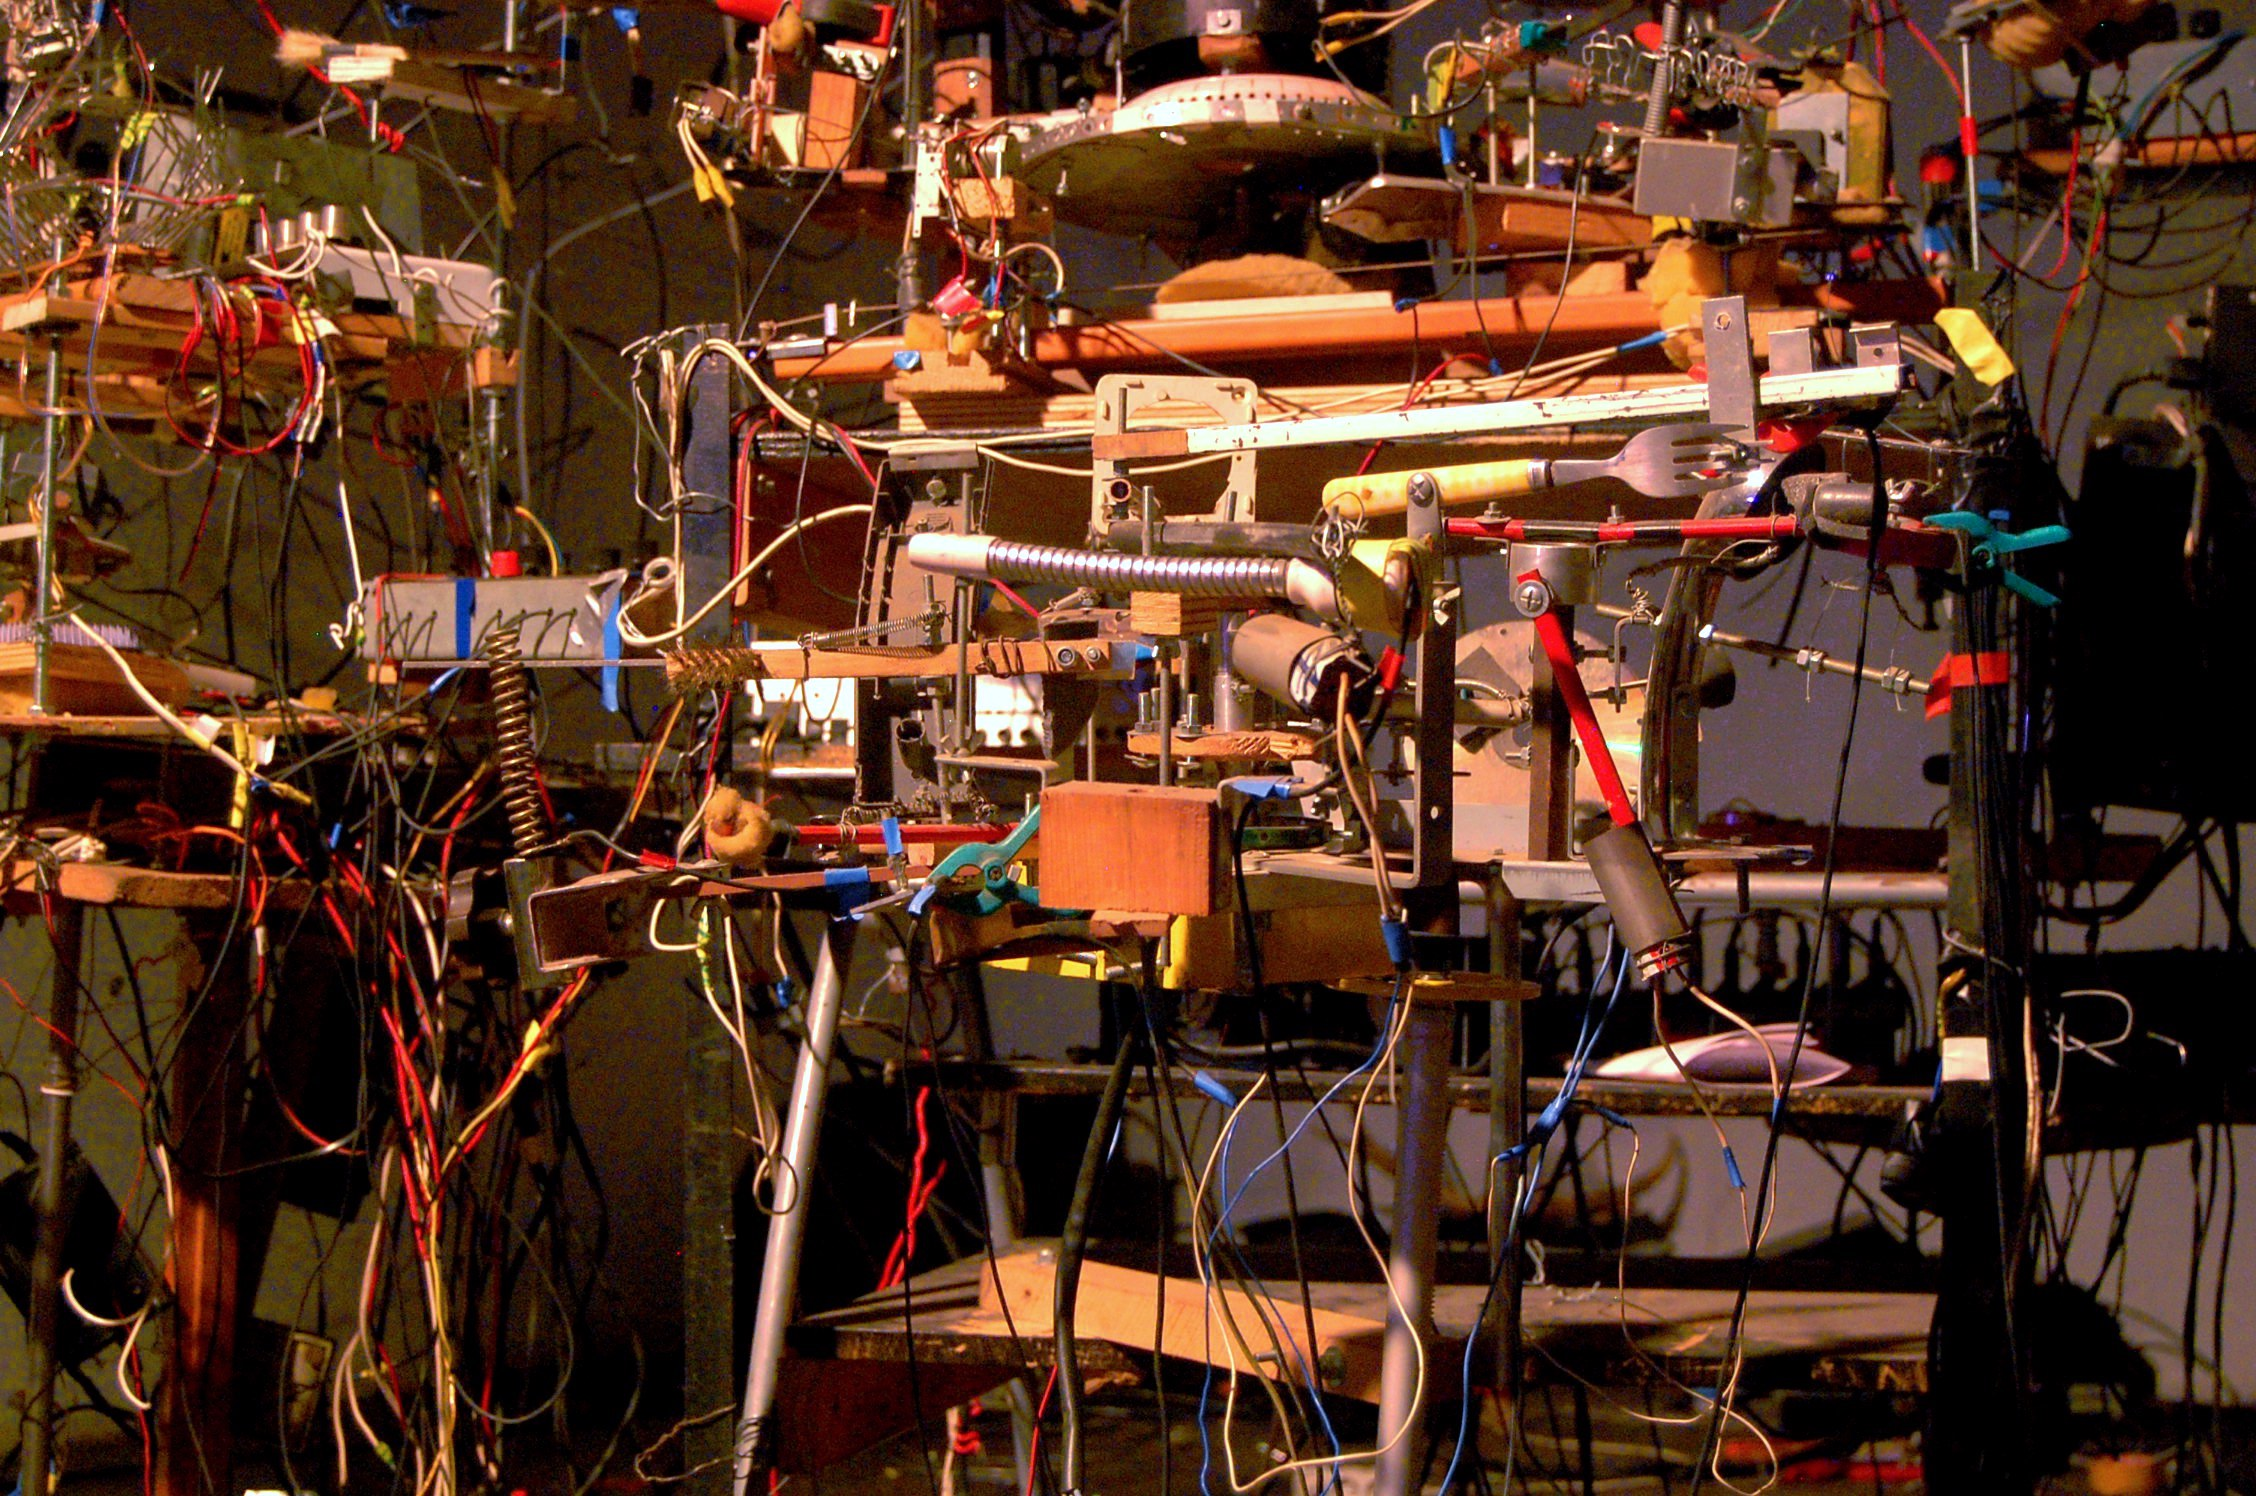
\includegraphics[width=\textwidth]{gfx/02_ephemeral/PierreGordeff.jpg}
	\caption[Détail d'un instrument de Pierre Gordeff]{Détail d'un instrument de Pierre Gordeff. Photographie : Pierre Gordeff}
	\label{fig:ephemeral:Gordeff}
\end{figure}

\subsection{Cuisiner des instruments à la volée}

\noindent Une autre raison qui contribue à la stabilité des instruments acoustiques est liée à leur physicalité et à leur fabrication, qui demande un travail considérable en regard de l'arrangement virtuel de blocs logiciels - la construction d'un violoncelle requiert plus de deux mois de travail pour un luthier qui connaît son métier ! A l'inverse, John Bowers et ses collaborateurs ont promu l'utilisation d'objets prêts à l'emploi comme ``infra-instruments'' semi-fabriqués \cite{bowers_not_2005} et comme instruments ``pin-and-play'' \textit{ad hoc} \cite{bowers_creating_2006}, en repensant le cycle de vie d'un instrument avec ce type de montage éphémère et rapidement assemblé.\\
\indent Plus généralement, lorsqu'on crée un \gls{DMI} avec un environnement de programmation audio, le logiciel fournit non seulement des fonctions de base mais aussi des bibliothèques, des exemples prêts à l'emploi, complétés par d'innombrables ressources en ligne, prêtes à être téléchargées, copiées et collées.\\
\indent Cela signifie que la conception d'un \gls{DMI} peut se faire très rapidement, de manière soustractive : plutôt que de partir d'une page blanche, il est possible de chercher une version proche de ce que l'on veut réaliser et de la modifier en partant de là. Nicolas Collins a comparé cette simplicité à la cuisine, en mettant l'accent sur sa démocratisation : \iquote{Ce que ça veut dire, c'est que si tu joues en live, si tu as vraiment besoin d'instruments spécialisés, cela s'apparente presque plus à de la cuisine qu'à de la fabrication d'instruments de musique. Tout le monde cuisine, tu n'as pas besoin d'aller dans une école pour chefs !} [Collins, communication personnelle, cf. annexe \ref{appendix:collins}]\\
\indent Les évolutions récentes des langages de programmation audio tendent à aborder la question de la durabilité en créant des langages spécifiques à un domaine qui peuvent être exportés vers différentes plateformes cibles. Des cartes électroniques comme \textit{Bela} ou \textit{The Owl}\footnote{Bela: \url{https://bela.io}; The Owl: \url{https://www.rebeltech.org}} et des langages comme \gls{FAUST} développé par le \gls{GRAME} \cite{orlarey_faust_2008} ou SOUL annoncé par Roli\footnote{Announced at the Audio Developer Conference 2018. \url{https://youtu.be/-GhleKNaPdk}} reflètent tous cette tendance. Il est intéressant de noter que \gls{FAUST}, qui a été conçu dans une optique de préservation, facilite en même temps la conception d'instances éphémères en offrant à la fois un compilateur en ligne et une compilation à la volée\footnote{En s'appuyant sur l'infrastructure \gls{LLVM}}.
	
\subsection{Une relation tri-partite: répertoire, musicien, contexte}

\noindent Si nous cessons de considérer l'éphémérité des instruments seulement comme un problème, nous pouvons envisager la manière dont longévité et éphémérité peuvent s'articuler dans l'agentivité des pratiques liées aux \glspl{DMI}. Celles-ci peuvent être envisagées comme un assemblage tripartite entre un ensemble de matériaux, un musicien et un contexte, chacun des membres présentant un degré différent de stabilité.

\subsubsection{Le grand répertoire}

\noindent Les composants d'un \gls{DMI} peuvent être considérés comme appartenant à un large répertoire patrimonial matériel et immatériel. Ce répertoire comprend notamment tous les matériaux physiques qui peuvent être utilisés dans la construction d'instruments acoustiques : matières premières, pièces usinées ou mécaniques. \\
\indent Le répertoire immatériel est l'ensemble des connaissances théoriques et du patrimoine culturel sur lesquels on peut s'appuyer lors de la fabrication d'un instrument\footnote{Bien évidemment, la connaissance pratique est aussi essentielle à la fabrication d'un instrument, même si elle n'appartient pas vraiment au patrimoine commun auquel je fais référence ici.} : théorie musicale, connaissances scientifiques et techniques, techniques de jeu établies, répertoire musical, etc. Cette connaissance oriente le façonnement des matériaux et guide leurs positionnements relatifs :  placement des frettes, accord des cordes, disposition des touches, etc.\\
\indent Dans le cas des \gls{DMI}, cependant, le répertoire des matériaux physiques est considérablement élargi par des connaissances réifiées disponibles sous forme de matériaux numériques, soit sous forme de code informatique, soit sous forme d'ensembles de données (e.g. échantillons audio, réponses impulsionnelles, séquences de notes, etc.) qui permettent de façonner l'identité et les qualités musicales d'un instrument au-delà de ce qui est possible avec les matériaux physiques. Cet ensemble, aussi hétérogène qu'il puisse paraître, constitue un répertoire partageable dans lequel les luthiers numériques peuvent puiser les ingrédients nécessaires à la conception de leur instrument.

\subsubsection{Le musicien \textit{in-progress} / \textit{in-process}}

\noindent Le deuxième élément de l'agencement est le musicien\footnote{Ici, le terme générique de ``musicien'' représente principalement l'instrumentiste, mais comme rappelé précédemment, les frontières entre les rôles d'instrumentiste, de compositeur et de luthier sont poreuses.}. Les musiciens sont vivants et sujets au changement : leurs connaissances, leur expérience et leurs désirs, leurs compétences et leur conscience musicale, leurs projets et leurs capacités physiques évoluent tout au long de leur existence. Cette évolution se reflète dans le dispositif instrumental, par l'ajout ou le retrait de composants, ou par le développement de nouveaux instruments liés à un nouveau projet musical. Ainsi, de même que l'on peut apprendre à conduire un vélo à l'aide de roues latérales et les enlever plus tard, les \glspl{DMI} se prêtent à une assistance évolutive pour un apprentissage progressif. Cette relation co-dynamique avec l'instrument peut aider à améliorer l'intimité\footnote{Sur la question du rapport d'intimité entre le musicien et un nouvel instrument, voir notamment les articles de Sydney Fels, e.g. \cite{fels_designing_2004}.} entre le musicien et l'objet technique qui devient instrument.

\subsubsection{Le \textit{hic et nunc} de la performance}

\noindent Enfin, le \gls{DMI} peut être adapté au contexte de la performance, qui est généralement plus éphémère que les deux aspects mentionnés ci-dessus.
En composant son propre répertoire musical à partir du grand répertoire susmentionné et de sa propre expérience, le musicien sélectionne un sous-ensemble d'éléments dans la perspective d'une performance particulière, pour une proposition artistique singulière et pour s'adapter aux conditions spatiales et temporelles de la performance, ainsi qu'au public. À titre d'exemple, le code qui se duplique sans peine offre des possibilités de redimensionner un instrument soliste en instrument collectif, en distribuant le contrôle sur plusieurs interfaces. De nouveaux projets peuvent impliquer de repartir de zéro, mais les projets existants n'impliquent souvent que des ajustements contextuels plutôt qu'une reprogrammation complète de son propre système. Chris Kiefer et Thor Magnusson ont proposé le terme de ``pre-gramming'' \cite{kiefer_live_2019} pour décrire ce type particulier de préparation\footnote{Dans le contexte du live-coding qui est le leur, Kiefer et Magnusson détournent en fait le terme ``pro-gramming'' pour désigner l'action de coder en live, face à un public, tandis que le ``pre-gramming'' est l'activité de programmation préalable à la ``pro-grammation''.}.
	

\section{Jouer d'un DMI éphémère}
\label{sec:ephemeral:playing-a-DMI}

\noindent Comme nous pouvons le voir, la création d'un \gls{DMI} peut être un processus très rapide, consistant en l'assemblage d'éléments déjà pré-construits. Mais une fois l'assemblage terminé, comment apprendre à en jouer ?

\subsection{Composer, concevoir, apprendre et jouer en parallèle}

\noindent Les instruments acoustiques traditionnels sont soutenus par des méthodes et un répertoire qui peuvent à leur tour s'appuyer sur la stabilité de l'instrument. Mais pour un nouveau \gls{DMI}, possiblement unique, possiblement éphémère, de telles ressources ne sont guère disponibles. Les logiciels sont au mieux livrés avec des manuels, mais ceux-ci expliquent généralement comment faire fonctionner le logiciel, pas comment jouer de la musique avec.\\
\indent De là, le processus d'apprentissage peut suivre deux directions apparemment opposées : trouver les bons gestes pour jouer les sons désirés et trouver les bons sons pour les gestes choisis. En conséquence, l'apprentissage d'un nouveau \gls{DMI} commence souvent dès sa conception et est un processus co-dynamique qui accompagne son développement jusqu'à la \textit{pré-grammation} de l'instrument, avec des allers-retours entre les moments de jeu et les moments de réglage. Ces allers-retours nécessitent de stopper le développement de l'instrument pour se consacrer entièrement au jeu comme le notait Michel Waisvisz : \iquote{La seule solution qui a fonctionné pour moi est de geler le développement technique pour une période de parfois presque deux ans, puis de me consacrer exclusivement à la composition, la performance et l'exploration/exploitation des limites [de l'instrument].}\footnote{``The only solution that worked for me is to freeze tech development for a period of sometimes nearly two years, and then exclusively compose, perform and explore/exploit its limits.'' dans \cite{wanderley_trends_2000}.}

\subsection{Entrer dans l'avenir à reculons}

\noindent Les \glspl{DMI} et leurs pratiques héritent du savoir-faire des musiques électroacoustiques thésaurisé depuis le milieu du \siecle{20}~siècle. La pédagogie de la musique électroacoustique s'est essentiellement appuyée sur les théories musicales de l'écoute \cite{schaeffer_traite_1966} et des métaphores pour composer \cite{bayle_musique_1993}, mais celles-ci furent conçues à une époque où la musique électroacoustique ne pouvait qu'être composée sur support, avant que les pratiques audio en temps réel ne permettent leur performance en live. En conséquence, ces théories étaient plus orientées vers la composition musicale que vers l'interprétation en tant que telle.\\
\indent En l'absence d'une notation musicale établie pour le son, la performance électronique expérimentale s'est en partie inspirée vers l'improvisation libre, qui implique un lâcher prise permettant à l'instrument d'exprimer ses potentialités et une pratique de ``l'auralité''\footnote{Décrite par Alain Savouret comme une théorie musicale pour l'audible.} pour ``entrer dans l'avenir à reculons'' \cite{savouret_introduction_2010} et réagir à ce qui sort de l'instrument plutôt que le maîtriser complètement. 
%\todo{Revoir ce paragraphe (cf discussion avec  Pierre)}

\subsection{Trouver les résonances}

\noindent L'apprentissage d'un instrument (au-delà de l'apprentissage des idiomes établis pour cet instrument) nécessite donc une recherche de résonance. On peut faire l'expérience de cette résonance à un niveau acoustique, mais plus généralement comme une résonance empathique, qui consiste à s'immerger dans l'instrument pour trouver les espaces qui vont (re)sonner de manière satisfaisante, pour trouver les \textit{sweet spots}\footnote{Il n'existe pas de véritable équivalent français pour cette expression anglaise, désignant un équilibre optimal, un réglage bien ajusté, une zone idéale. Les ingénieurs du son l'utilisent notamment pour désigner l'emplacement d'écoute idéale par rapport à la position des haut-parleurs.} où ce que nous entendons rencontre ce que nous cherchions, parfois sans le savoir. La linéarité mathématique étant rarement satisfaisante au niveau perceptuel, cette exploration impliquant la coordination entre le jeu et l'écoute critique est essentielle pour ajuster les fonctions de transfert qui vont définir le comportement de l'instrument.

\subsection{Pratique modulaire de la stabilité}

\noindent Si l'agencement éphémère d'un \gls{DMI} peut sembler trop instable pour pouvoir établir des méthodes pédagogiques pérennes, ses composantes individuelles peuvent offir des points d'accroche plus stables. Par exemple, si la performance est basée sur une partition écrite, l'instrumentiste peut apprendre l'enchaînement des gestes appropriés nécessaires à sa réalisation\footnote{La pièce ``Aphasia'' de Mark Applebaum (https://youtu.be/wWt1qh67EnA), où la performance repose sur des gestes et une bande sonore totalement notés, en est un exemple radical de ce point de vue là.}.\\
\indent En ce qui concerne le comportement du \gls{DMI}, on peut en partie transférer sa connaissance d'autres \glspl{DMI} à une nouvelle instance qu'on essaie d'apprendre. Par exemple, l'intégration d'une synthèse \gls{FM} dans un \gls{DMI} peut aider une personne familière avec ce type de synthèse à naviguer dans son espace timbral. Elle y retrouvera l'espace sonore caractéristique de la \gls{FM}\footnote{J'entend par là non seulement les différents timbres (cloches, sirènes, cuivres, etc.) caractéristique de cette synthèse, mais également la topologie de leur répartition dans l'espace paramétrique}, indépendamment de l'interface de contrôle qui y est branchée, en s'appuyant sur ses propres connaissances et représentations de l'espace de paramètres de la synthèse \gls{FM}. L'espace de timbre de diverses synthèses audio peut également être redistribué sur un espace perceptif commun et plus stable (en s'appuyant par exemple sur des paramètres perceptifs tels que la hauteur, le volume, la brillance, etc.) qui dissocie leur contrôle des différents espaces de paramètres respectifs, tels que présentés dans \cite{wessel_timbre_1979}, \cite{arfib_strategies_2002}, \cite{schwarz_sound_2012} ou \cite{tubb_divergent_2014}.

\indent En 1999, Jean-Claude Risset écrivait dans \cite{genevois_les_1999} : \iquote{La disponibilité `d'accès' gestuels tout à fait différents des accès instrumentaux risque de rester lettre morte, dans la mesure où il est improbable que des interprètes réalisent l'investissement considérable que représente l'apprentissage d'un instrument complètement nouveau s'ils n'ont pas l'assurance que cet instrument va durer et qu'un répertoire va se développer pour lui.} On comprend aisément l'avertissement de Risset quand on le met en perspective de l'investissement des musiciens classiques, ainsi que des traditions instrumentales parfois pluri-centenaires. Son analyse omet toutefois de considérer la métamorphose que traverse la notion de répertoire, que Risset semble associer à la tradition de l'œuvre notée sur partition et destinée à un instrument spécifique, dont la pratique sera enseignée dans un conservatoire, et qui connut son apogée à l'époque romantique.\\
\noindent Pourtant, on voit les pratiques se développer malgré cette situation incertaine et instable, et une expertise peut être acquise sur une nouvelle interface sensible\footnote{Sur la notion d'interface sensible, cf. chapitre \ref{ch:interfaces}}, qui invite à des gestes et des déplacements spécifiques\footnote{Par exemple, la scène musicale du \textit{launchpad} s'est développée autour d'une interface particulière, le launchpad de Novation, qui doit en partie son succès à son prix abordable et sa simplicité d'usage (absence de vélocité \gls{MIDI}, une seule prise \gls{USB}, dédié au logiciel Ableton Live). Cette interface qui consiste uniquement en une matrice d'interrupteurs On/Off --~à la différence des Pads de batterie, sensible à la vélocité et prévus pour des gestes percussifs~-- a connu l'appropriation de toute une communauté d'utilisateurs. Les affrontements de virtuosité rythmique et la possibilité de programmer dynamiquement les couleurs (et le mapping) du launchpad en a fait un phénomène Internet, à travers la publication de \textit{remixes} et de \textit{mashups} virtoses sur YouTube (e.g. \textit{Marble Soda} de Shawn Wasabi \url{https://youtu.be/qAeybdD5UoQ}). L'émergence de cette scène a donné lieu à un certain nombre de tutoriels vidéos pour apprendre à jouer, ainsi qu'à des logiciels pédagogiques dédiés (e.g. Melodics, ``a desktop app that teaches you to play MIDI keyboards, pad controllers, and MIDI drum kits.'' \url{https://melodics.com/})} ; cette expertise repose sur une mémoire spatiale incorporée, qui reste en partie indépendante des synthèses ou effets audio contrôlés par l'interface. La stabilité comportementale de l'instrument peut également être de nature virtuelle, par exemple en utilisant des modèles intermédiaires dynamiques \cite{goudard_dynamic_2011} (cf. \ref{sec:algorithms:MID}), qui peuvent servir de référence stable entre diverses synthèses et interfaces en évolution.
\noindent Dans l'ensemble, cette connaissance transposée et ``modulaire'' ne peut fournir que les grandes lignes de ce qui est nécessaire à la pratique subtile d'un instrument. Le diable se cache évidemment dans les détails.


\subsection{Entomologie musicale}
\label{sec:ephemeral:vessels}

\noindent L'exploration musicale d'un \gls{DMI} fait surgir des formes musicales inconnues, comme des papillons éphémères. L'apprentissage d'un \gls{DMI} implique donc souvent une tâche similaire à celle de l'entomologiste, qui consiste à épingler ces créatures sonores et à leur donner un nom. Ce nommage permettra d'y revenir plus tard (en les sauvegardant dans des presets par exemple) ainsi que de discuter avec d'autres musiciens d'une performance qui, en l'absence d'idiomes musicaux établis sur lesquels s'appuyer, comme les gammes ou la signature temporelle, peut cruellement manquer de références. Une telle tâche a été menée dans le développement de ``John, le semi-conducteur'', un système de partition ouvert décrit dans \cite{goudard_john_2018} et dans le chapitre \ref{ch:notation}.\\
%-------------------------- Figure : Entomologie ----------------------------------
\begin{figure}[!htbp]
	\captionsetup{format=plain}%
	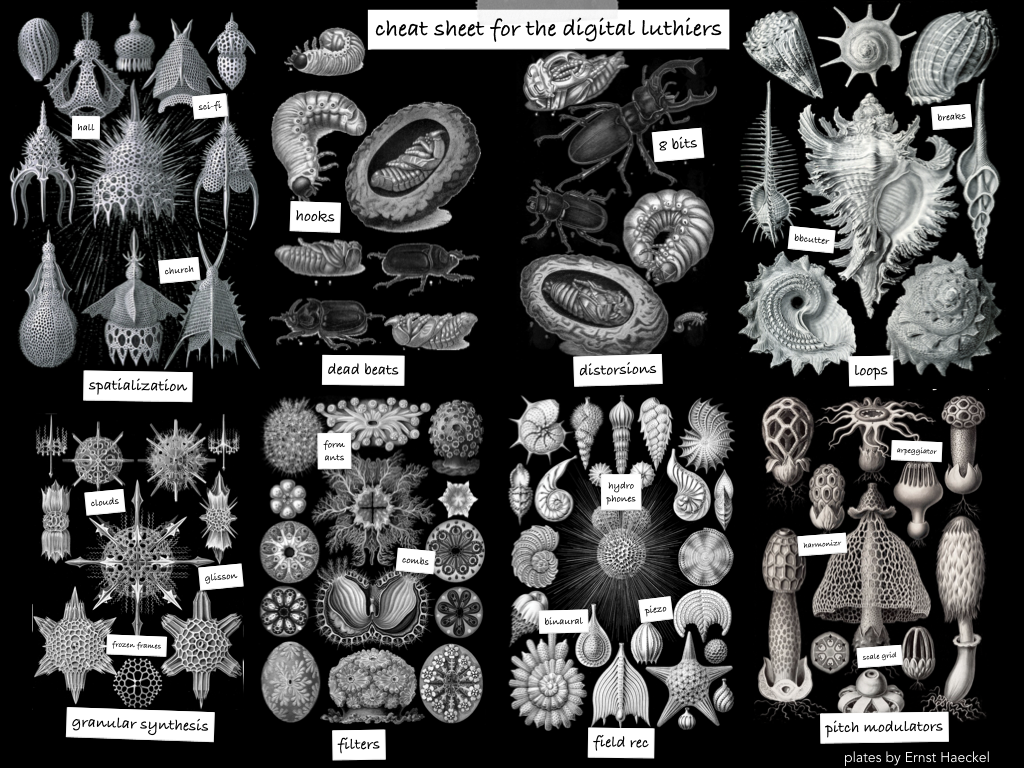
\includegraphics[width=\textwidth]{gfx/02_ephemeral/Bestiaire.png}
	\caption{Entomologie musicale}
	\label{fig:ephemeral:entomologie}
\end{figure}
%-------------------------- Figure : Entomologie ----------------------------------
\noindent Les \glspl{DMI} s'apparentent ainsi à des vaisseaux hétérogènes, chargés de souvenirs de nos expériences d'interprétation, de composition ou de fabrication d'instruments. Les sons que nous recueillons, les algorithmes de synthèse que nous développons (ou téléchargeons), les paramètres que nous ajustons, les recettes de cuisine et les fonctions de transfert que nous élaborons avec soin, contribuent à l'évolution d'un répertoire personnel où se cristallisent des instances éphémères. Thor Magnusson a proposé le terme ``d'outil épistémique'' pour décrire les \glspl{DMI} comme \iquote{un outil conçu avec un tel degré de pertinence symbolique qu'il devient un système de connaissance et de pensée dans ses propres termes} \cite{magnusson_epistemic_2009}.\\
\indent Ainsi, les \glspl{DMI} se présentent comme des assemblages évolutifs de ces matériaux enregistrés et impliquent souvent des activités qui ne sont généralement pas associées à la pratique instrumentale, comme la gestion de fichiers, le versionnage du code, le recensement de ressources en ligne ou l'organisation de banques de sons, afin de pouvoir réunir ces ressources aussi rapidement que possible pour la performance.\\
\indent Il est remarquable que les possibilités de duplication et de diffusion offertes par les médias numériques et Internet n'aient pas conduit à la standardisation des instruments ; les \glspl{DMI} sont souvent très personnels et singuliers.

\section{Conclusion}

\noindent Ce chapitre a permis de présenter les \glspl{DMI} à travers la notion d'assemblage éphémère qui les caractérise, en la considérant non pas seulement comme un problème, mais comme une modalité intrinsèque de leur ontologie. Loin d'exclure leur longévité, elle éclaire au contraire la conception technique des environnements propices à leur développement et à leur durabilité.\\
\indent L'éphémérité des outils n'empêche pas la production de musique passionantes, ni la réalisation de performances musicales captivantes. Au contraire, elle peut à la fois favoriser l'adaptation des assemblages musicaux à des contextes essentiellement éphémères et défier la capacité de l'être humain à répondre à un dispositif musical fugace et indompté.\\
\indent Il y a un millénaire, l'émergence de la notation musicale a entraîné une multiplication du nombre de compositions, dont un grand nombre connurent une vie éphémère en terme de performances. Le numérique nous amène peut-être aujourd'hui à une situation similaire en ce qui concerne l'instrument : la possibilité de le ``noter'' sous forme de code donne lieu à une multiplication du nombre de nouveaux instruments. En mettant cette révolution en perspective de celle que fût l'écriture musicale il y a un millénaire, et de qu'elle permit en terme de création de forme (de l'\textit{ars antiqua} à l'écriture symphonique), on peut espérer que la \textit{notation instrumentale} soit aussi fertile.\\
\indent En fin de compte, les œuvres musicales (et les instruments) semblent trouver leur chemin, qu'on les appelle ``répertoire classique'', ``standard de jazz'' ou ``airs traditionnels'', mais ce n'est pas tant la pérennité de leur notation qui les fait survivre --~elles pourraient rester \textit{lettre morte}~--, que l'intérêt que leur portent les vivants, qui soutiennent par leurs soins et leur travail celles qu'ils reconnaissent comme chefs-d'œuvre. Elles peuvent résister à l'épreuve du temps en étant dispersées, distribuées, transformées, recomposées, réinterprétées ou même renommées, par tous ceux qui y attacheront de l'importance. Ce soin attentionné, mû par notre désir de musique, appartient probablement à la partie de notre mémoire que nous ne pouvons pas externaliser dans un outil et qui redéfinit la tradition et la préservation en dehors du cadre technologique.\\
\indent Dans le sable évoqué par Michel Chion, nous pouvons voir une autre métaphore intéressante pour les \glspl{DMI}: à l'origine, le sable est une roche, qui s'est progressivement atomisée, fragmentée en particules infimes. La même chose semble s'être produite pour les instruments de musique, atomisés en petits modules numériques. Nous pouvons jouer avec le sable comme un matériau fluide, ou lui ajouter de l'eau, voire du ciment, pour lui donner une forme concrète.\\
\indent Si les technologies numériques arrivent un jour à maturité, nous pourrons peut-être compter sur des instruments numériques stables et durables. Dans ce cas, et faisant suite à la prémonition de Garsault, il ne faudra pas oublier de classer tous les instruments éphémères qui les ont précédés dans la catégorie des \iquote{instruments hors d'usage, mais qui peuvent revenir}.


%\section{extra material}

% Thor Magnusson in Sonic Writing (p12) : Anyone who plays a musical instrument will be familiar with the special moment when a new instrument is picked and its ergodynamics studied through play. (footnote : we often change our instruments during performance : we retune string instruments, change effect settings in electronics, and the \textit{whole point} of live coding is to create and redefine the instrument during play). This experience of ergodynamics recognises that an instrument is an object that never rests, or enter a period of stasis: that every time we pick it up there are new things to discover, new patterns our fingers know, because we have changed, the instrument has changed, and so has the whole world itself — the general performance context.

% De même que l'histoire a connu une importance prépondérante des musiques traditionnelles\footnote{Les musiques trad existent toujours, et d'une certaine manière, un standard de jazz est une musique traditionnelle}, à une époque où l'absence d'écriture et d'enregistrement rendait cette tradition nécessaire à la répétition, la période allant du Moyen-Age à l'époque contemporaine a été marqué par la prépondérance d'instruments traditionnels, à défaut de pouvoir agencer ces instruments de manière plus souple, comme l'a permis l'écriture pour la composition musicale. La possibilité de ``noter'' ces instruments sous forme de grammes, ainsi que les gestes ne rend plus nécessaire l'existence de tradition instrumentale, ou plutôt, rend plus que jamais possible l'invention instrumentale.

% De même que l'on peut travailler une partition et devenir expert dans son interprétation, on peut travailler un instrument pour en devenir expert et travailler les différentes compositions pour cet instrument. On peut aujourd'hui travailler le geste (et l'écoute!) et en devenir expert pour jouer les différents instruments qui s'offrent à ces gestes.